\documentclass[12pt,a4paper]{article}

\makeatletter
\def\input@path{{/home/maenwe/Master_CSM/modèle_cours_latex}}
\makeatother

\usepackage{prise_de_note}

\begin{document}
	
	\begin{titlepage}
		\centering
		
		% Logo
		\begin{figure}[h]
			\centering
			% Ajustez la largeur si besoin (ex: 0.4 ou 0.6)
			
\includegraphics[width=0.5\textwidth]{logo.jpg} 
		\end{figure}
		
		\vspace{2cm}
		
		% Filet horizontal du haut
		\rule{\linewidth}{0.5mm} \\[0.4cm]
		
		% Titre
		{\color{bleuTitre} \Huge \bfseries Cours} \\[0.4cm]
		
		% Filet horizontal du bas
		\rule{\linewidth}{0.5mm}
		
		\vspace{1.5cm}
		
		{\Large \textbf{Modélisation en action}}
		
		\vfill
		
		% Bloc Informations
		\begin{minipage}{0.45\textwidth}
			\begin{flushleft} \large
				\textbf{Enseignant :} \\
				M. Christophe \textsc{DROZ}
			\end{flushleft}
		\end{minipage}
		\hfill
		\begin{minipage}{0.45\textwidth}
			\begin{flushright} \large
				\textbf{Étudiant :} \\
				Nathan \textsc{HASCOET}
			\end{flushright}
		\end{minipage}
		
		\vspace{2cm}
		
		% Date
		{\large \today}
		
	\end{titlepage}
	
	\tableofcontents
	
	\newpage
	
	\section{Introduction à la théorie de Floquet-Bloch}
	\subsection{Équation d'onde dans un milieu continu périodique}
	
	Considérons l'aquation d'ondes se propageant dans un milieu homogène où la vitesse $c$ est une fonction de la position $x$ : $\frac{\partial^2 U}{\partial t^2} = \frac{\partial}{\partial x} \left(c(x)^2 \frac{\partial U}{\partial x}\right)$.
	
	\par On se place en \textbf{\underline{régime harmonique}} (stationnaire en temps).\\\\
	En substituant dans l'équation (substituant), on obtient :
	\begin{center}
		\fbox{
			$\frac{d}{dx}\left(c(x)^2 \frac{dU}{dx}\right) + \omega^2 u = 0$ que l'on note $\mathcal{L}_{\omega}u = 0$.
		}
	\end{center}
	,où $\mathcal{L}_{\omega}u$ est l'opérateur (différentiel) qui reflète l'équilibre dynamique (ou équilibre des forces) en toute position $x$ à la fréquence $\omega$.
	
	\begin{center}
		\fbox{$\mathcal{L}_{\omega}u$ encode les lois physique : $\mathcal{L}_{\omega}u = \frac{d}{dx}\left(c(x) ^2\frac{d \cdot}{dx}\right) + \omega^2$.}
	\end{center}
	
	$\longrightarrow$ Considérons désormais que \textbf{$c$} est une fonction $P$-périodique, c'est à dire \fbox{$c(x+P) = c(x)$}.
	
	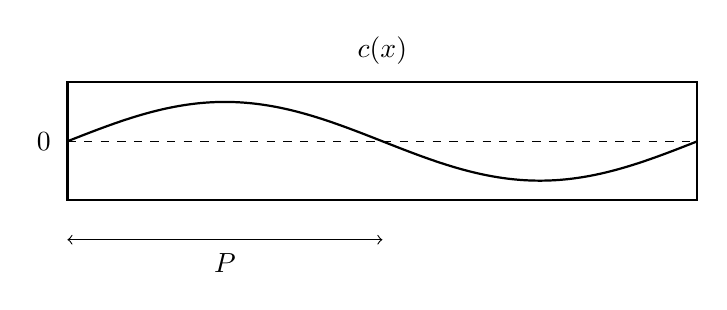
\begin{tikzpicture}[scale=1]
		
		% Rectangle (domaine périodique)
		\draw[thick] (0,0) rectangle (8,1.5);
		
		% Axe x implicite
		\draw[dashed] (0,0.75) -- (8,0.75);
		
		% Courbe périodique c(x)
		\draw[thick,domain=0:8,samples=200]
		plot (\x,{0.75 + 0.5*sin(180*\x/4)});
		
		% Indication de la période P
		\draw[<->] (0,-0.5) -- (4,-0.5);
		\node at (2,-0.8) {$P$};
		
		% Labels
		\node at (4,1.9) {$c(x)$};
		\node at (-0.3,0.75) {$0$};
		
	\end{tikzpicture}
	
	On note $\mathcal{T}\mathcal{}$ l'opérateur de translation de $p$ défini par, pour toute fonction $V$ : $\left(\mathcal{T} v\right)(x) = v(x + P)$ ($v$ est suffisamment régulier).
	
	$\longrightarrow$ \textbf{Nous allons montrer que} $\mathcal{L}_\omega$ et $\mathcal T$ \textbf{commutent}, c'est-à-dire : $\left[\mathcal L_\omega, \mathcal T\right] := \mathcal L_\omega \mathcal T - \mathcal T \mathcal L_\omega = 0$.
	
	C'est à dire pour toute fonction $v$, \fbox{$\mathcal L_\omega\left(\mathcal T v\right) = \mathcal T \left(\mathcal L_\omega v\right)$}.
	
	\begin{enumerate}
		\item[$(1)$] $\begin{aligned}[t]
			\mathcal L_\omega(\mathcal T v)(\lambda)
			&= \mathcal L_\omega(v(\cdot + P))(\lambda) \\
			&= \frac{d}{dx}(c(x)^2 v'(x+P)) + \omega^2 v(x+P) \\
			&= 2c(x)c'(x)v'(x+P) + c(x)^2 v''(x+P) + \omega^2 v(x+P).
		\end{aligned}$
		
		\vspace{.2cm}
		
		\item[$(2)$]  $\begin{aligned}[t]
			\mathcal T \left(\mathcal L_\omega v\right)(x) 
			&= \left(\mathcal L_\omega v\right)(x+P)\\
			&= \frac{d}{dy}\left(c(y)^2v'(y)\right) + \omega^2v(y)\\
			&= 2c'(y)c(y)v'(y) + c(y)^2v''(y) + \omega^2v(y) \\
			&= (2)
		\end{aligned}$
		, où $y = x + p$.
	\end{enumerate} 
	
	Les deux expressions (1) et (2) sont identiques.
	
	\subsection{Invariance translationnelle et ondes de Bloch}
	
	Puisque $\mathcal L_\omega$ et $\mathcal T$ commutent, ils partagent une base de fonctions propres. (cf. théorème spectral pour les opérateurs commutants). Considérons l'espace des solutions $\ker\left(\mathcal L_\omega\right) = \left\{u, \mathcal L_\omega v = 0\right\}$. Il est invariant par $\mathcal T$ et par commutation on peut diagonaliser simultanément :\\
	Il existe des solutions qui sont à la fois dans $\text{Ker}(\mathcal L_\omega)$, et qui sont fonctions propres de $\mathcal T$.\\
	
	\textit{\underline{Remarque :}} Fonction propre de $\mathcal T v = \lambda v, \lambda \in \mathbb{R}$\\
	
	\begin{minipage}{8cm}
		Cela se traduit par : \fbox{$u(x+P) = \lambda u(x)$}.
	\end{minipage}
	\begin{minipage}{8cm}
		\textit{Cette forme correspond à des ondes de Bloch (ondes planes modulées dans le milieu périodique).}
	\end{minipage}
	
	Les solutions sont propagatives si $|\lambda| = 1$ et évanescentes si $|\lambda| \not =  1$.
	
	\subsection{Généralisation aux opérateurs différentiels en dimension N}
	On considère l'opérateur de $\mathbb{R}$ sur $\mathbb{C}^N$ :
	\[
	\mathcal L v = \sum_{k = 0}^n [A]_k(x) \frac{d^k v}{dx^k}, \quad 
	\text{où } 
	\begin{cases}
		\forall x, & [A]_k(x+P) = [A]_k(x),\\
		& [A]_k \text{ : matrice } \mathbb{C}^{N\times N}.
	\end{cases}
	\]
	
	
	L'opérateur de translation est $\left(\mathcal T v\right)(x) = v(x+P)$. De nouveau, si$\mathcal L et \mathcal T$ commutent , alors ils admettent des fonctions propres (communes) et les solutions $u$ de $\mathcal L v = 0$ peuvent être choisi tels que : $\mathcal T v = \lambda v$ $\implies$ $c(x+P) = \lambda v(x)$ où $\lambda \in \mathbb{C}$ est une valeur propre scalaire de $\mathcal T$.
	\begin{enumerate}
		\item[$(i)$] $\begin{aligned}[t]
			\mathcal L\left(\mathcal T v\right)(x) 
			&= \sum_{k=0}^n [A]_k(x) \frac{d^k}{dx^k}\left(\mathcal T v\right)(x)\\
			&= \sum_{k=0}^n [A]_k(x) \, v^{(k)}(x+P)
		\end{aligned}$\\
		
		\item[$(ii)$] $\begin{aligned}[t]
			\mathcal T\left(\mathcal L v\right)(x) 
			&= \left(\mathcal L v\right)(x+P)\\
			&= \displaystyle\sum_{k=0}^n [A]_k(x+P)v^{(k)}(x+P)\\
			&= (i)
		\end{aligned}$
	\end{enumerate}
	
	Donc $\left[\mathcal L, \mathcal T\right] = 0$.\\
	Les deux précédents opérateurs sont des EDP et concernent des systèmes périodiques continus. Nous allons considérer dans la suite des systèmes discrets.
	
	\subsection{Opérateurs périodiques continus vs. opérateur discrétisés}
	
	Pour simplifier, considérons le système d'ordre $n = 2$.
	\[
	A_2(x)u^{(2)}(x) + A_1(x)u^{(1)} + A_0(x)u(x) = 0
	\]
	
	\vspace{-.5cm}
	
	où les $A_i$ sont des matrices $N\times N$.\\
	On discrétise $x$ sur la grille \[\begin{cases}
		u_n = u(x_n)\\
		x_n = nh
	\end{cases}\] 
	On approxime $u^{(i)}$ par différences finies.
	\[
	u_n^{(1)} = \frac{u_{n+1} - u_{n-1}}{2h} \text { et } u_n^{(2)} = \frac{u_{n+1}-2u_n+u_{n-1}}{h^2}
	\]
	L'opérateur discrétisé devient :
	\[
	A_2(x_n)\left(\frac{u_{n+1}-2u_n+u_{n-1}}{h^2}\right) + A_1(x_n)\left(\frac{u_{n+1}-u_{n-1}}{2h}\right) + A_0(x_n)u_n = 0
	\]
	
	On multiplie par $h^2$ et on regroupe les $u_{n+1}, u_n, u_{n-1}$ et on note $A_1(n) := A(x_n)$.
	
	\[
	\left[A_2(n) + \frac{h}{2} A_1(n)\right]u_{n+1} + \left[h^2A_0(n) - 2A_2(n)\right] u_n + \left[A_2(n) - \frac{h}{2} A_1(n)\right]u_{n-1} = 0
	\]
	
	On note : $B_1(n) = A_2(n) + \frac{h}{2} A_1(n)$, $B_0(n) = h^2A_0(n) - 2A_2(n)$ et $B_{-1}(n) = A_2(n) - \frac{h}{2} A_1(n)$.\\
	
	Puisque $A_k(x+P)  =A_k(x)$, nous avons $A_k(n+M) = A_k(n)$ et donc $B_k(n+M) = B_k(n)$ est $m$-périodique.\\
	
	$\longrightarrow$ \textit{\textbf{On supposera}} que $B_1$ est inversible pour que la récurence soit explicite.\\\\
	Notons $\mathcal T$ l'opérateur de translation discret : $\left(\mathcal T u\right) = u(n-M) := u_{n+1}.$\\
	
	\vspace{-.5cm}
	
	\underline{\textbf{Démontrons que} $\left[\mathcal L, \mathcal T\right] = 0$ :} $\left(\mathcal L v\right)(n) = B_1(n)u_{n+1} = B_0(n)u_n + B_{-1}(n)u_{n-1}$\\
	
	Calculons : $\begin{aligned}[t]
		\mathcal T\left(\mathcal L v\right)(n) 
		&= \left(\mathcal L u\right)(n+M)\\
		&= B_1(n+M)u_{n+M+1} + B_0(n+M)u_{n+M} + B_{-1}(n+M)u_{n+M-1}\\
		\text{\scalebox{0.7}{\textit{où $B$ est périodique  }}} &= B_1(n)u_{n+m-1} + B_0(n)u_{n+M} + B_{-1}(n)u_{n+M-1}\\
		&= \mathcal L\left(\mathcal T v\right)(x) 
	\end{aligned}$
	
	\fbox{
		\begin{minipage}{15cm}
			Les solutions sont donc des ondes de Bloch discrète, c'est-à-dire de la forme :
			
			$u_n = e^{\mu n}\phi(n)$, où :
			\[
			\begin{cases}
				\phi \text{ est } M\text{-périodique }(\text{i.e. } \phi(n+M) = \phi(n))\\
				\mu \in \mathbb{C} \text{ est l\'exposant de Floquet}
			\end{cases}
			\]
		\end{minipage}
	}
	
	Cela implique $\begin{aligned}[t]
		\left(\mathcal T u\right)(n) 
		&:= u_{n+M} \\
		&= e^{\mu(n+M)}\\
		&=  e^{\mu n}e^{\mu M}\phi(n)\\
		&= e^{\mu M}u_n
	\end{aligned}$
	\hspace{1cm} On note \underline{$\lambda = e^{\mu M}$}.
	
	\hspace{-1cm}\begin{minipage}[t]{20cm}
		Ainsi $\left(\mathcal T u\right)(x) = \lambda u_n$ ce qui revient à dire que c'est un vecteur propre de $\mathcal T$ et $\lambda$ est valeur propre, est dit "Multiplicateur de Floquet".
	\end{minipage}
	
	\subsection{Interprétation des constantes de propagation}
	
	Notation pour le milieu périodique :
	\[
	\begin{cases}
		P = M a\\
		x_n = na
	\end{cases}; u(x_n+P) = u(na+Ma) := u_{n+M}
	\]
	
	\begin{prop}$ $\\
		
		\begin{minipage}{20cm}
			\fbox{
				\begin{minipage}{14.5cm}
					\begin{tabular}{l|l}
						\begin{minipage}{7cm}
							\underline{En 'continue' :}\\
							$u(x+P) = \lambda u(x)$ avec $\lambda = e^{ikP}$\\
							$\iff$\\
							$u(x) = e ^{ikx}\phi(x)$, avec $\phi(x+P) = \phi(x)$\\
							
							où $k\in \left[\frac{-\pi}{P},\frac{\pi}{P}\right] \left(\frac{2\pi}{P}\right)$ "Nombre d'onde"
						\end{minipage}
						& 
						\begin{minipage}{7cm}
							\underline{En 'discret' :}\\
							$u_{n+1} = \lambda u_n$ avec $\lambda = e^{ikMa}$\\
							$\iff$\\
							$u_n = e^{ikna}\phi(n)$, avec $\phi(n+M) = \phi(n)$\\
							
							où $k\in \left[\frac{-\pi}{Ma},\frac{\pi}{Ma}\right] \left(\frac{2\pi}{Ma}\right)$
						\end{minipage}
					\end{tabular}
				\end{minipage}
			} \begin{minipage}{2cm}
				\textcolor{blue}{\textit{Forme des solutions}}
			\end{minipage}
		\end{minipage}
	\end{prop}
	
	\begin{dem}
		\underline{En 'continue' :}\\
		\begin{minipage}[t]{10cm}
			Montrons que (1) $\implies$ (2).\\
			$\begin{aligned}
				u(x) = e^{-ikP}u(x+P) 
				&= e^{ikx} \underbrace{e^{ik(x+P)}u(x+P)}_{\phi(x+P)}\\
				&=e^{ikx} \underbrace{e^{-ikx}\phi(x)}_{\phi(x)}
			\end{aligned}$
		\end{minipage}\begin{minipage}[t]{12.5cm}
			Montrons que $(2) \implies (1)$.\\
			$\begin{aligned}
				u(x+P) 
				&= e^{ik(x+P)}\phi(x+P)\\
				&= e^{ikP}e^{ikx}\phi(x) \text{ , car } \phi \text{ est périodique}\\
				&= \fbox{$e^{ikP}u(x)$}
			\end{aligned}
			$
		\end{minipage}
		
		\vspace{.5cm}
		
		Le cas 'discret' se fait de la même manière.
	\end{dem}
	
	Ces formes de solutions caractérisent la propriété d'une onde se propageant dans un milieu périodique, continu ou discret.
	
	\textbf{\textit{Nous supposerons}} l'existence de cette forme de solution en invoquant le Principe de Floquet-Bloch.
	
	\subsection{Nombre d'onde et constante de propagation}
	
	\begin{enumerate}
		\item[$\cdot$] Si $|\lambda| = 1$ les ondes sont propagatives 
		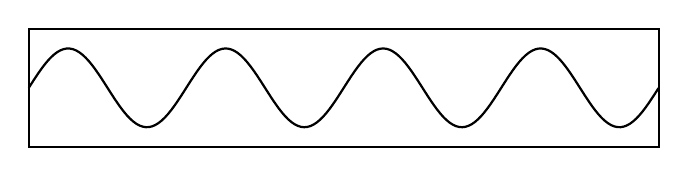
\begin{tikzpicture}[scale=1]
			
			% Rectangle (domaine périodique)
			\draw[thick] (0,0) rectangle (8,1.5);
			
			% Courbe périodique c(x)
			\draw[thick,domain=0:8,samples=200]
			plot (\x,{0.75 + 0.5*sin(180*\x)});
			
		\end{tikzpicture}
		
		\item[$\cdot$] Si $|\lambda| < 1$ les ondes sont évanescentes progressives
		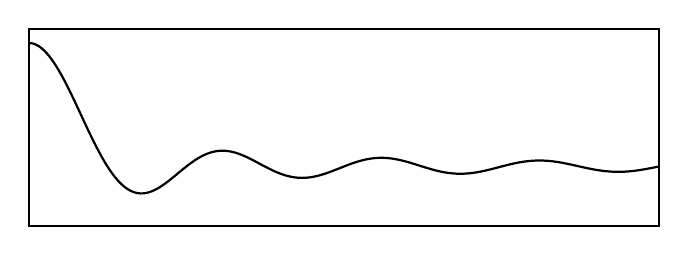
\begin{tikzpicture}[scale=1]
			
			% Rectangle (domaine périodique)
			\draw[thick] (0,0) rectangle (8,2.5);
			
			% Courbe périodique c(x)
			\draw[thick,domain=0.01:8,samples=200]
			plot (\x,{0.75 + 0.5*sin(180*\x)/\x});
			
		\end{tikzpicture}
		
		\item[$\cdot$] Si $|\lambda| > 1$ les ondes sont évanescentes régressive
		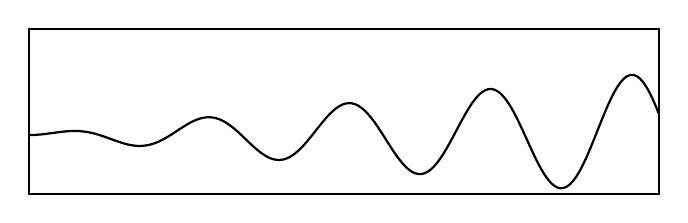
\begin{tikzpicture}[scale=1]
			
			% Rectangle (domaine périodique)
			\draw[thick] (0,0) rectangle (8,2.1);
			
			% Courbe périodique c(x)
			\draw[thick,domain=0.01:8,samples=200]
			plot (\x,{0.75 + 0.1*\x*sin(200*\x)});
			
		\end{tikzpicture}
	\end{enumerate}
	
	\[
	\begin{aligned}
		\text{Comme } u(x + nP) 
		&= \lambda^nu(x) = e^{iknP}u(x) &\text{, or } k = \operatorname{Re}(k) + i\operatorname{Im}(k)\\
		&= e^{-\operatorname{Im}(k)nP}e^{i\operatorname{Re}(k)nP}u(x)
	\end{aligned}
	\]
	
	
	
	\[
	\underbrace{U(x+nP)}_{\textcolor{red}{\text{Translation spatial}}} =\quad
	\underbrace{e^{-\operatorname{Im}(k)nP}}_{\textcolor{red}{\text{Décroissance spatiale}}}\cdot
	\underbrace{e^{i\re(k)nP}}_{\textcolor{red}{\text{Changement de phase}}}\cdot \quad u(x)
	\]
	
	On utilisera les valeurs de $k \in \mathbb{C}$ pour classifier, tracer et interpréter les ondes.
	
	En rappelant que $U(x,t) = \operatorname{Re}\left(u(x,t)e^{-i\omega t}\right)$, on peut donner la forme des solutions dans un milieu $P$-périodique infini comme :\\
	$U(x,t) = U_n(x,t) = \operatorname{Re}\left(u_0(\omega)e^{-i\omega t}\right)$ qui s'écrit d'après le principe de Floquet-Bloch :
	
	\vspace{-.1cm}
	
	\begin{minipage}{6cm}
		\begin{tcolorbox}[colback=white, colframe=red, arc=1mm, boxrule=1pt]
			$U_n(t) = \operatorname{Re}\left(u_0(\omega)e^{i(nkp-\omega t)}\right)$
		\end{tcolorbox}
	\end{minipage} , où $u_0(\omega)$ est l'amplitude de l'onde.\\
	
	\textbf{$\longrightarrow$ Dans la suite}, nous chercherons à trouver les valeurs de $k$ (\textbf{relation de dispersion}) pour différents systèmes périodique (discrets ou continu/discrétisés par éléments finis)
	
	\section{Modélisation dynamique des systèmes périodique discrets}
	
	\subsection{Chaîne monoatomique}
	
	COnsidérons un système infini constitué d'atomes de masse $m$, espacés d'une distance $a$ et reliés par des raideurs linéaires (ressort, quoi) de constante $\beta$.\\
	
	
\includegraphics[scale=.5]{photo1.png}
	
	Ecrivons l'équation d'équilibre d'u atome au point $x_n$ (en l'indice $n$)
	\[
	m\dfrac{d^2U_n}{dt^2} = \displaystyle\sum F_{\text{ext}} = -\beta(U_n-U_{n+1}) - \beta(U_n-U_{n-1}) = \beta(U_{n+1}-2U_n+U_{n-1})
	\]
	
	\textbf{En régime stationnaire} $U_n(t) = u_n(\omega)e^{i\omega t}$.\\
	Principe de Floquet-Bloch : $U_n(t) = u_0(\omega)e^{i(\omega t - kna)}$\\
	
	
	L'équation d'équilibre devient : 
	
	\[
	\begin{aligned}
		m\omega^2 \cancel{U_0e^{i(\omega t - kna)}} 
		&= \beta \left(e^{ika}-2 + e^{-ika}\right)\cancel{U_0e^{i(\omega t - kna)}}\\
		m\omega^2 
		&= \beta \left(e^{ika}-2 + e^{-ika}\right) = 2\beta\left(\frac{e^{ika}+e^ {-ika}}{2}-1\right) = 2\beta\left(\cos(ka)-1\right)\\
		&= - 4\beta \sin^2\left(\frac{ka}{2}\right)
	\end{aligned}
	\]
	
	Donc$\omega^2 = \frac{4\beta}{m}\sin^2\left(\frac{ka}{2}\right)$, en notant $\omega_0 = 2 \sqrt{\frac{\beta}{m}}$, on obtient : \fbox{$\omega = \omega_0\left|\sin\left(\frac{ka}{2}\right)\right|$},\\
	qui est la relation de dispersion, sous la forme $\omega(k)$.\\
	
	\fbox{
		\begin{minipage}[t]{18.5cm}
			\textbf{\underline{Représentation de la solution:}}\\
			
			\begin{minipage}{10cm}
				
\includegraphics[scale=.3]{photo2.png}
			\end{minipage}\begin{minipage}[t]{8cm}
				Comme $k$ est $\frac{2\pi}{a}$-périodique, on ne représente les solution que dans l'intervalle $\left[\frac{-\pi}{a},\frac{\pi}{a}\right]$.
			\end{minipage}
			
			Connaissant le nombre d'onde $k$, on détermine $\begin{cases}
				\text{la vitesse de phase } C_p = \frac{\omega}{k}\\
				\text{la vitesse de groupe } c_z = \frac{\partial \omega}{\partial k}
			\end{cases}$
			
			
\includegraphics[scale=.5]{photo3.png}
			
			$\longrightarrow$ Paquet d'ondes : superposition d'ondes progressives dans un intervalle $k$.
	\end{minipage}}
	
	\vspace{.5cm}
	
	\par \textbf{Cherchons} les solutions complexes $k(\omega)$.
	
	Reprenons : $-\omega^2m = \beta\left(e^{ika}+e^{-ika}-2\right) = 2\beta \left(\frac{e^{-ika}+e^{ika}}{2} - 1 \right)$
	
	$-2\omega^2 = \underbrace{\frac{4\beta}{m}}_{\omega_0^2}\left(\frac{e^{ika}+e^{ika}}{2} - 1\right)$, on introduit : $\begin{cases}
		\lambda = e^{ika}\\
		\lambda^{-1} = e^{-ika}
	\end{cases}$ 
	
	$\dfrac{\lambda+\lambda^{-1}}{2} - 1 + 2 \dfrac{\omega^2}{\omega_0^2} = 0 \implies \fbox{$\lambda^2 + \left(4\dfrac{\omega^2}{\omega_0^2}-2\right)\lambda + 1 = 0$}$
	
	$\Delta = \left(4\dfrac{\omega^2}{\omega_0^2}-2\right)^2-4 = 16\dfrac{\omega^4}{\omega_0^4} - 16 \dfrac{\omega^4}{\omega_0^2} = 16\dfrac{\omega^2}{\omega_0^2}\left[\dfrac{\omega^2}{\omega_0^2} - 1\right]$\\
	
	\begin{minipage}[t]{8cm}
		On reconnais le cas où $\omega \leq \omega_0$ ($\Delta < 0$) :
		
		\[
		\fbox{$
			\lambda = 1 - 2 \dfrac{\omega^2}{\omega_0^2} \pm 2i \dfrac{\omega}{\omega_0}\sqrt{1-\dfrac{\omega^2}{\omega_0^2}}
			$}	
		\]
	\end{minipage}\hspace{1cm}\begin{minipage}[t]{5cm}
		\fbox{\rouge{!}} Si $\lambda_1$ est solution alors $\lambda_2 = \frac{1}{\lambda_1}$ l'est aussi
	\end{minipage}
	
	
	On a 3 cas celons les valeur de $\omega$ et $\omega_0$.
	\begin{enumerate}
		\item Lorsque $\omega > \omega_0$, il n'y a pas de solution propagative, les ondes sont évanescentes :
		\[
		\fbox{
			$
			\lambda = 1 - 2 \dfrac{\omega^2}{\omega_0^2} \pm 2 \dfrac{\omega}{\omega_0} \sqrt{\dfrac{\omega^2}{\omega_0^2}-1}
			$
		}
		\]
		
		Pour retrouver les solutions explicites $k(\omega)$ on peut utiliser : 
		\[
		\begin{aligned}
			\lambda 
			&= e^{ika} = e^{i\left(\re(k)+i\im(k)\right)a} = e^{i\re(k)a}e^{-\im(k)a}\\
			&= e^{-k_I a }\cos(k_R a) + i e^{-ik_I a}\sin(k_R a)
		\end{aligned}
		\]
		
		\item Lorsque $\omega \leq \omega_0$, $\cos(k_Ra) = 1-2\frac{\omega^2}{\omega_0^2}$ et $\sin^2(\frac{k_R a}{2}) = \frac{\omega^2}{\omega_0^2}$.
		
		\item Lorsque $\omega > \omega_0$, on a $\lambda \in \R$, donc $k_R = \pm \frac{\pi}{a} \left[2\pi\right]$.
	\end{enumerate}
	
	\vspace{.5cm}
	
	\par Donc $\lambda = \pm e^{-k_I a} = \pm \left[1-2\frac{\omega^2}{\omega_0^2} \pm2\frac{\omega^2}{\omega_0^2}\sqrt{\frac{\omega^2}{\omega_0^2}-1}\right]$
	
	Donc $k_I = \frac{1}{a}\log\left(-1+2\frac{\omega^2}{\omega_0^2} \pm \frac{2\omega}{\omega_0}\sqrt{\frac{\omega^2}{\omega_0^2}-1}\right)$\\
	
	\textbf{Calcul de :} $\begin{aligned}[t]
		\left(\Omega+\sqrt{\Omega^2-1}\right)
		&= \Omega^2 + 2\Omega\sqrt{\Omega^2 -1} + \Omega^2-1\\
		&=-1 + 2\omega^2+2\Omega\sqrt{\Omega^2-1}
	\end{aligned}$\\
	
	\textbf{Calcul de :} $\begin{aligned}[t]
		\left(\Omega-\sqrt{\Omega^2-1}\right)
		&= \Omega^2 - 2\Omega\sqrt{\Omega^2 -1} + \Omega^2-1\\
		&=-1 + 2\omega^2-2\Omega\sqrt{\Omega^2-1}
	\end{aligned}$
	
	\vspace{.2cm}
	
	\hrule
	
	\vspace{.5cm}
	
	$k_I = \frac{1}{a}\log\left[-1 + 2\frac{\omega^2}{\omega_0^2} - 2\frac{\omega}{\omega_0^2}\sqrt{\frac{\omega^2}{\omega_0^2}-1}\right]$
	
	
\includegraphics[scale=.6]{photo4.png}
	
	\textbf{\underline{Conclusions :}}
	\begin{enumerate}
		\item[$\cdot$] $\omega(k)$ est plus facile à détermier, mais ne donne pas les solutions évanescentes (c'est-à-dire $\im(k)$).
		\item[$\cdot$] $k(\omega)$est plus difficile à calculer mais donne la signification physque de l'évanescence à l'intérieur de la bande interdite.
	\end{enumerate}
	
	\newpage
	
	\subsection{Chaîne di-atomique}
	
	Considérons le système discret périodique à deux atomes :
	
	
\includegraphics[scale=.5]{photo5.png}
	
	Ecrivons l'équation d'équilibre de la cellule unitaire (i.e. l'élément qui, répété, permet de reconstituer toute la chaîne).
	
	\[
	\begin{aligned}
		m_1\dfrac{d^2U_n}{dt^2} = -\beta\left(U_n-V_n\right) - \beta\left(U_n-V_{n-1}\right)\\
		m_2\dfrac{d^2V_n}{dt^2} = -\beta\left(V_n-U_{n-1}\right) - \beta\left(V_n-U_n\right)
	\end{aligned}
	\]
	
	On considère le régime stationnaire et on applique le principe de Floquet-Bloch : 
	\[
	\begin{aligned}
		u_n = u_0e^{i(\omega t - kna)} = u_0\lambda^n e^{i\omega t}\\
		v_n = v_0 e^{i(\omega t-kna)} = v_0\lambda^ne^{i\omega t}
	\end{aligned}
	\]
	En injectant dans les équations d'équilibre on obtient :
	\[
	\begin{aligned}
		\text{(1) }\omega^2 m_1  U_0 
		&= 2\beta\left(U_0-\frac{V_0}{2}-\frac{1}{\lambda}\frac{V_0}{2}\right)
		\begin{cases}
			u_{n+1} = \lambda u_n\\
			u_{n-1} = \frac{1}{\lambda} u_n
		\end{cases}
		\text{ et }
		\begin{cases}
			v_{n+1} = \lambda v_n\\
			v_{n-1} = \frac{1}{\lambda} v_n
		\end{cases}\\
		\text{(2) }\omega^2 m_2V_0 
		&= 2\beta\left(V_0-U_0-\lambda \frac{U_0}{2}\right)
	\end{aligned}
	\]
	
	$(1)/m_1$ avec $\omega_1 = \sqrt{\frac{2\beta}{m_1}}$ et $(2)/m_2$ avec $\omega_2 = \sqrt{\frac{2\beta}{m_2}}$ :
	$\begin{cases}
		\omega^2U_0-\omega_1^2\left(U_0-\frac{V_2}{2}-\frac{1}{\lambda}\frac{V_0}{2}\right) = 0\\
		\omega^2V_0-\omega_2^2(V_0-\frac{U_0}{2}-\frac{\lambda}{2}U_0) = 0
	\end{cases}$
	
	Ce système  s'écrit sous forme matricielle :
	\[
	\left[\begin{matrix}
		\omega^2 - \omega_1^2 & \frac{\omega_1^2}{2}(1+\frac{1}{\lambda}) \\
		\frac{\omega_2^2}{2}(1+\lambda) & \omega^2-\omega_2^2
	\end{matrix}\right]\left[\begin{matrix}
		U_0\\
		V_0
	\end{matrix}\right] = \left[\begin{matrix}
		0\\
		0
	\end{matrix}\right]
	\]
	
	Les solutions sont non-triviales pour Det = 0 c'est-à-dire :
	\[
	\begin{aligned}
		(\omega^2-\omega_1^2)(\omega^2-\omega_2^2) - \frac{\omega_1\omega_2}{4}(1+\frac{1}{\lambda})(1+\lambda) = 0\\
		\omega^4 - \omega^2(\omega_1^2+\omega_2^2)-\frac{\omega_1^2\omega_2^2}{4}(2+\lambda+\frac{1}{\lambda}) + \omega_1^2\omega_2^2
	\end{aligned}\]
	
	On remarque que $\lambda + \frac{1}{\lambda} = e^{-ika}+e^{ika} = 2 \cos(ka)$\\
	$\omega^4-\omega^2(\omega_1^2+\omega_2^2) - \frac{\omega_1^2\omega_2^2}{4}(\lambda+\frac{1}{\lambda}-2) = 0$.\\
	Donc $\lambda+\frac{1}{\lambda} = 2\cos(ka) - 2 = -4\sin^2(\frac{ka}{2})$.\\
	Ainsi on peut écrire :
	\[
	\omega^4-\omega^2(\omega_1^2+\omega_2^2) - \omega_1^2\omega_2^2\sin^2(\frac{ka}{2}) = 0
	\]
	
	Et $\Delta = (\omega_1^2+\omega_2^2)^2 - \omega_1^2\omega_2^2\sin^2(\frac{ka}{2})$ positif car $\sin ^2 \leq 1$ et $(\omega_1^2-\omega_2^2)^2 \geq 0$.\\
	Les deux solutions s'écrivent :
	\[
	\omega^2(k) = \beta \left(\frac{1}{m_1}+\frac{1}{m_2}\right) \pm \beta \sqrt{\left(\frac{1}{m_1}+\frac{1}{m_2}\right)^2-\frac{4\sin^2(\frac{ka}{2})}{m_1m_2}}
	\]
	on introduit $\omega_3 = \sqrt{2\beta\left(\frac{1}{m_1}+\frac{1}{m_2}\right)} =: \omega_{max}$.\\
	
	
\includegraphics[scale=.5]{photo6.png}
	
	Si on suppose que $m_1=m_2$, la relation de dispersion devient : $\omega^2(k) = \omega_1^2(1\pm\cos(\frac{ka}{2}))$.\\
	Intéressons-nous désormais aux propriétés de l'ondes à l'intérieur de la bande interdite :\\
	Reprenons la relation de dispersion :
	\[
	\begin{cases}
		\omega^2U_0 = \omega_1^2\left(U_0-\frac{V_2}{2} -\frac{1}{\lambda}\frac{V_0}{2}\right) & /\omega_1 ^2 \text{ et } \Omega_1 ^2 = \frac{\omega^2}{\omega_1^2} \\
		\omega^2V_0 = \omega_2^2(V_0-\frac{U_0}{2} -\frac{\lambda}{2}U_0) & /\omega_2^2 \text{ et } \Omega_2^2 = \frac{\omega^2}{\omega_2^2}
	\end{cases}
	\begin{cases}
		(2\Omega_1^2-2)U_0 + (1+\frac{1}{\lambda})V_0 = 0 \\
		(1+\lambda)U_0+(2\Omega_2^2-2)V_0 = 0
	\end{cases}
	\]
	
	On annuler le déterminant :
	\[
	\begin{aligned}
		(2\Omega_1^2-2)(\Omega_2^2-2) - \underbrace{(1+\frac{1}{\lambda})(1+\lambda)}_{\rouge{4\sin^2(\frac{ka}{2})}} = 0\\
		\lambda - \underbrace{\left[4(\Omega_1^2-1)(\Omega_2^2-1) +2\right]}_{2(1-2(\Omega_1^2-1)(\Omega_2^2-1))} + \frac{1}{\lambda} = 0\\
		\Delta = 16(\Omega_1 ^2-1)(\Omega_2^2-1)\left[\underbrace{(\Omega_1^2-1)(\Omega_2^2-1)}_{\rouge\Gamma}-1\right]
	\end{aligned}
	\]
	
	Les solutions complexes sont alors :
	\[
	\lambda = (2\Gamma-1)\pm2\sqrt{(\Omega_1^2-1)(\Omega_2^2-1)(\Gamma-1)}
	\]
	
	\fbox{
		\begin{minipage}[t]{15cm}
			Ce qui donne la solution $k(\omega)$ explicite :
			\[
			k(\omega) = \frac{i}{a}\log\left[\frac{1}{\omega_1^2\omega_2^2}\left(2\omega^4-2\omega^2\omega_3^2 + \omega_1 ^2\omega_2^2 + 2\omega\sqrt{(\omega^2-\omega_1^2)(\omega^2-\omega_2^2)(\omega^2-\omega_3^2)}\right)\right]
			\]
	\end{minipage}}
	
	
	\hspace{-.5cm}
\includegraphics[scale=.4]{photo7.png}
	
	\subsection{Généralisation aux systèmes à plusieurs degrés de liberté (DDL)}
	
	On considère une chaîne masse-ressort :
	
	
\includegraphics[scale=.5]{photo11.png}
	
	L'équation d'équilibre en régime harmonique s'écrit en $U_n$ :
	
	\[m_n\dfrac{d^2U_n}{dt^2} = -\beta_n(U_n-U_{n+1}) - \beta_{n-1}(U_n-U_{n-1})\]
	
	qui s'écrit : $m_n \overset{\textbf{..}}{U}_n - \beta_{n-1}U_{n-1} + (\beta_n+\beta_{n-1})U_n - \beta_nU_{n+1} = 0$.\\
	Le système s'écrit sous forme matricielle :
	\[\left[\begin{matrix}
		\ddots & & & & \\
		& m_{n-1} & & (0) & \\
		& & m_n & & \\
		&(0) & & m_{n+1} & \\
		& & & & \ddots
	\end{matrix}\right]\left[\begin{matrix}
		\vdots\\
		\overset{\textbf{..}}{U}_{n-1}\\
		\overset{\textbf{..}}{U}_{n}\\
		\overset{\textbf{..}}{U}_{n+1}\\
		\vdots
	\end{matrix}\right] + \left[\begin{matrix}
		\ddots & & & & \\
		& \ddots & & & \\
		(0) & - \beta_{n-1} & \beta_{n+1}+\beta_n & -\beta_n & (0)\\
		& & & \ddots & \\
		& & & & \ddots
	\end{matrix}\right]\left[\begin{matrix}
		\vdots\\
		U_{n-1}\\
		U_n\\
		U_{n+1}\\
		\vdots
	\end{matrix}\right] = \left[\begin{matrix}
		0 \\
		\vdots \\
		\vdots \\
		\vdots \\
		0
	\end{matrix}\right]\]
	
	C'est une EDO qui s'écrit : 
	\begin{center}
		\begin{minipage}{4cm}
			\enc{red}{$\mathbb{M}\dfrac{\partial^2 \overset{\rightarrow}{U}}{\partial t^2} + \mathbb{K} \overset{\rightarrow}{U} = \overset{\rightarrow}{0}$}
		\end{minipage}
	\end{center}
	
	On \textbf{nomme} \underline{$\mathbb{M}$ la \textbf{matrice de masse}} et \underline{$\mathbb{K}$ la \textbf{matrice de raideur}}.
	
	\newpage
	
	On peut représenter l'écriture des matrices $\mathbb{K}$ et $\mathbb{M}$ du système comme un "assemblage" d'éléments discrets (raideurs 1D) qui sont des cellules :\\
	\newlength{\x}
	\setlength{\x}{1cm}
	\newlength{\y}
	\setlength{\y}{1.5cm}
	\[\mathbb{K} = \left[\begin{matrix}
		-\beta_{n-1} & \beta_{n-1}+\rouge{\beta_n} & \rouge{-\beta_n} & 0 &  \\
		0 & \rouge{-\beta_n} & \rouge{\beta_n} + \bleu{\beta_{n+1}} & \bleu{-\beta_{n+1}} & 0 \\
		& 0 & \bleu{\beta_{n+1}} & \bleu{\beta_{n+1}} + \beta_{n+2} & - \beta_{n+2}
	\end{matrix}\right]\]
	
	Cela permet d'écrire de façon plus rapide les matrices (EDO) d'un système périodique :
	
	\begin{ex}\begin{minipage}{15cm}
			
\includegraphics[scale=.5]{photo12.png}
		\end{minipage}
		
		Écrire le système (EDO) sous la forme $\mathbb{M}\overset{\textbf{..}}{U} + \mathbb{K}U = 0$.
		
		\begin{minipage}[t]{19.5cm}
			\textbf{\underline{Rappel :}} \begin{minipage}{3cm}
				
\includegraphics[scale=.5]{photo13.png}
			\end{minipage} le système est : $\left[\begin{matrix}
				m_1 & 0 \\
				0 & m_2
			\end{matrix}\right] \left[\begin{matrix}
				\overset{\textbf{..}}{U} \\ 
				\overset{\textbf{..}}{V}
			\end{matrix}\right] + \left[\begin{matrix}
				k & -k \\
				-k & k
			\end{matrix}\right]\left[\begin{matrix}
				U \\
				V
			\end{matrix}\right] = \left[\begin{matrix}
				0 \\ 0
			\end{matrix}\right]$.
		\end{minipage}
		
		\vspace{.5cm}
		
		\[
		\left[\begin{matrix}
			\rouge{m_1} & 0 & 0 & 0 \\
			0 & m_2 & 0 & 0 \\
			0 & 0 & m_3 & 0 \\
			0 & 0 & 0 & m_4
		\end{matrix}\right]\left[\begin{matrix}
			\overset{\textbf{..}}{U_1} \\ \overset{\textbf{..}}{U_2} \\ \overset{\textbf{..}}{U_3} \\ \overset{\textbf{..}}{U_4}
		\end{matrix}\right] + \left[\begin{matrix}
			\rouge{k_1} + k_4 & \rouge{-k_1} & 0 & -k_4 \\
			\rouge{-k_1} & \rouge{k_1}+\bleu{k_2} & \bleu{-k_2} & 0 \\
			0 & \bleu{-k_2} & \bleu{k_2} + \Vert{k_3} & \Vert{-k_3} \\
			-k_4 & 0 & \Vert{-k_3} & \Vert{k_3} + k_4
		\end{matrix}\right]\left[\begin{matrix}
			U_1 \\ U_2 \\ U_3 \\ U_4
		\end{matrix}\right] = \left[\begin{matrix}
			0 \\ 0 \\ 0 \\ 0
		\end{matrix}\right]
		\]
		
		En régime stationnaire , $\mathbb{M}\overset{\rightarrow}{\overset{\textbf{..}}{U}} + \mathbb{K}\overset{\rightarrow}{U} = \overset{\rightarrow}{0}$ devient : $ \underbrace{\left(\mathbb{K}-\omega^2\mathbb{M}\right)}_{\rouge{\mathbb{D}}}U = 0$. Où $\rouge{\mathbb{D}}$ est la raideur dynamique.		
	\end{ex}
	
	
	\begin{ex}\begin{minipage}{18cm}
			
\includegraphics[scale=.5]{photo14.png}
		\end{minipage}
		
		\begin{enumerate}
			\item Écrire les matrices $\mathbb{K}, \mathbf{M}$ d'une cellule périodique "bords libres".
			
			\[
			\underbrace{\left[\begin{matrix}
					\frac{m_1}{2} & 0 & 0 \\
					0 & m_2 & 0 \\
					0 & 0 & \frac{m_1}{2}
				\end{matrix}\right]}_{\mathbb{M}}\left[\begin{matrix}
				\overset{\textbf{..}}U_L \\ \overset{\textbf{..}}U_i \\ \overset{\textbf{..}}U_R 
			\end{matrix}\right] + \underbrace{\left[\begin{matrix}
					\rouge{k_1} & \rouge{-k_1} & 0 \\
					\rouge{-k_1} & \rouge{k_1} + \bleu{k_2} & \bleu{-k_2} \\
					0 & \bleu{-k_2} & \bleu{k_2}
				\end{matrix}\right]}_{\mathbb{K}}\left[\begin{matrix}
				U_L \\ U_i\\ U_R
			\end{matrix}\right] = \left[\begin{matrix}
				0 \\ 0 \\ 0
			\end{matrix}\right]
			\]
			
			qui s'écrit : $\left(\mathbb{K}-\omega^2\mathbb{M}\right)\left[\begin{matrix}
				U_L \\ U_i \\ U_R
			\end{matrix}\right] = \left[\begin{matrix}
				0 \\ 0 \\ 0
			\end{matrix}\right]$.
			
			Utilisons $\mathbb{K}$ et $\mathbb{M}$ pour écrire l'EDO du système "généralisé" : 
			
			\[\left(\left[\begin{matrix}
				\bleu{k_1}+\bleu{k_2} & \bleu{-k_2} & & \\
				\bleu{-k_2} & k_1 + \bleu{k_2} & -k_1 & 0 \\
				& -k_1 & k_1+k_2 & -k_2 \\
				& 0 & -k_2 & k_2+k_1
			\end{matrix}\right] -\omega^2\left[\begin{matrix}
				\bleu{m_2} & & & \\
				& \frac{m_1}{2}+\bleu{\frac{m_1}{2}} & & \\
				& & m_2 & \\
				& & & \frac{m_1}{2}+\frac{m_1}{2}
			\end{matrix}\right]\right)\left[\begin{matrix}
				\vdots\\
				\left[\begin{matrix}
					U_L^{(n)}\\
					U_i^{(n)}
				\end{matrix}\right] \\
				\vdots
			\end{matrix}\right] = \left[\begin{matrix}
				\vdots\\
				\left[\begin{matrix}
					0\\
					0
				\end{matrix}\right] \\
				\vdots
			\end{matrix}\right]\]
			
			
			On obtient :
			
			\[
			\left(\left[\begin{matrix}
				0 & -k_2 & k_1 + k_2 & -k_1 & 0& 0 \\
				0 & 0 & -k_1 & k_1 + k_2 & -k_2 & 0
			\end{matrix}\right]-\omega^2\left[\begin{matrix}
				0 & 0 & m_1 & 0 & 0 & 0 \\
				0 & 0 & 0 & m_2 & 0 & 0
			\end{matrix}\right]\right)\left[\begin{matrix}
				U_L^{(n-1)} \\
				U_i^{(n-1)} \\
				U_L^{(n)} \\
				U_i^{(n)} \\
				U_L^{(n-1)} \\
				U_i^{(n-1)}
			\end{matrix}\right] = \left[\begin{matrix}
				0 \\
				\vdots \\
				0
			\end{matrix}\right]
			\]
		\end{enumerate}
		
		
\includegraphics[scale=.5]{photo15.png}
	\end{ex}
	
	
	\begin{ex}[Poutre d'Euler-Bernoulli] Éléments discrets\\
		\begin{minipage}{7cm}
			
\includegraphics[scale=.5]{photo16.png}\\
			$\rho$ : densité volumique \\
			$A$ : Section \\
			$L$ : longueur \\
			$I$ : Moment de section \\
			$E$ : Module de Young
		\end{minipage} $ \begin{aligned}
			\mathbb{M}_e =& \dfrac{\rho A L}{420}\left[\begin{matrix}
				156 & 22L & 54 & -13L \\
				& 4L^2 & 13L & -3L^2 \\
				& & 156 & -22L \\
				& & & 4L^2
			\end{matrix}\right] \\
			\mathbb{K}_e =& \dfrac{2EI}{L}\left[\begin{matrix}
				6 & 3L & -6 & 3L \\
				& 2L^2 & -3L & L^2 \\
				&     & 6 & -3L \\
				(Sym) &   &   & 2L^2
			\end{matrix}\right]
		\end{aligned} $
		
		On peut décomposer nos matrices élémentaires en deux "domaines" (c'est-à-dire $U_L, U_R$) : $\mathbb{M}_e = \left[\begin{matrix}
			M_L & M_{LR} \\
			M_{RL} & M_R
		\end{matrix}\right]$ et $\mathbb{K}_e = \left[\begin{matrix}
			K_L & K_{LR} \\
			K_{RL} & K_R
		\end{matrix}\right]$.\\
		\begin{minipage}[t]{18cm}
			Où, par symétrie de $\mathbb{M}_e$ et $\mathbb{K}_e$ : $\begin{cases}
				M_L = M_L^T & \text{ (idem pour } M_R, K_L, K_R) \\
				M_{LR} = M_{RL}^T & \text{ (idem pour } K_{LR} = K_{RL}^T)
			\end{cases}$\\
			
			On note alors les raideurs dynamiques : $D_{i,j} = K_{i,j}-\omega^2M_{i,j}$, $i,j \in \{L,R\}$.
		\end{minipage}
		
		\underline{Le système initial :} 
		
		\vspace{.5cm}
		
		\begin{minipage}[t]{18.5cm}
			$\left(\mathbb{K}_e-\omega^2\mathbb{M}_e\right)\overset{\rightarrow}{U} = 0$ alors : $\left[\begin{matrix}
				D_L & D_{LR} \\
				D_{RL} & D_R
			\end{matrix}\right]\left[\begin{matrix}
				\overset{\rightarrow}{U_L} \\ \overset{\rightarrow}{U_R}
			\end{matrix}\right] = \left[\begin{matrix}
				0 \\ 0
			\end{matrix}\right]$, où $\overset{\rightarrow}{U_L} = \left[\begin{matrix}
				V_L \\ \Theta_L
			\end{matrix}\right]	$ et $\overset{\rightarrow}{U_R} = \left[\begin{matrix}
				V_R \\ \Theta_R
			\end{matrix}\right]	$
		\end{minipage}
		
		\begin{minipage}[t]{16cm}
			Écrivons l'assemblage de deux cellules décrites par leur matrice de raideur dynamique : $\mathbb{D} = \left[\begin{matrix}
				D_L & D_{LR} \\
				R_{RL} & D_R
			\end{matrix}\right]$ \begin{minipage}{5cm}
				
\includegraphics[scale=.5]{photo17.png}
			\end{minipage}
		\end{minipage}
		
		\[
		\left[\begin{matrix}
			\rouge{D_L} & \rouge{D_{LR}} & \\
			\rouge{D_{RL}} & \rouge{D_R}+D_L & D_{LR} \\
			& D_{RL} & D_R
		\end{matrix}\right]\left[\begin{matrix}
			U_L^{n-1} \\ U_L^n \\ U_L^{n+1}
		\end{matrix}\right] = \left[\begin{matrix}
			0 \\ 0 \\ 0
		\end{matrix}\right]
		\]
		Pour un assemblage "infini" de cellules :\\
		\begin{minipage}[t]{18.5cm}
			$\left[\begin{matrix}
				\ddots & \ddots & \ddots & & & & \\
				& D_{RL} & D_L+D_R & D_{LR} & & & & \\
				& \ddots & \ddots & \ddots & & & \\
				& & D_{RL} & D_L+D_R & D_{LR} & & \\
				& & & \ddots & \ddots & \ddots & \\
				& & & & D_{RL} & D_L + D_R & D_{LR} \\
				& & & & \ddots & \ddots & \ddots
			\end{matrix}\right]\left[\begin{matrix}
				\vdots \\
				U_{n-1} \\
				U_n\\
				U_{n+1} \\
				\vdots
			\end{matrix}\right] = \left[\begin{matrix}
				\vdots \\ \vdots \\ 0 \\ \vdots \\ \vdots
			\end{matrix}\right]$
		\end{minipage}
	\end{ex}
	
	
	\textbf{\underline{Comment traiter les cellules avec des nœuds interne ?}}\\
	
	
\includegraphics[scale=.8]{photo21.png}\\
	
	Écrivons la matrice de masse : $\mathbb{M} = \left[\begin{matrix}
		\frac m2 \\
		& M\\
		& & \frac m2
	\end{matrix}\right]$\\
	La matrice de raideur est : $\mathbb{K} = \left[\begin{matrix}
		K & -K \\
		-K & K+K & -K \\
		& -K & K
	\end{matrix}\right]$\\
	La raideur dynamique : $\mathbb{D} : \left[\begin{matrix}
		K-\omega^2 \frac m2 & -K & 0 \\
		-K & 2K-\omega^2 M & -K \\
		0 & -K & K-\omega^2\frac m2
	\end{matrix}\right]\left[\begin{matrix}
		U_L\\U_i\\U_R
	\end{matrix}\right]=\left[\begin{matrix}
		0 \\ 0 \\ 0
	\end{matrix}\right]$.\\
	Nous allons substituer $U_i$ par $U_L$ et $U_R$ :\\
	$\begin{aligned}
		(2) & -KU_L-KU_R+(2K-\omega^2 M)U_i = 0 \implies U_i = \dfrac{KU_L+KU_R}{2K-\omega^2M}\\
		(1) \implies &  (K-\omega^2\frac m2)U_L-K\left(\dfrac{K_L+KU_R}{2K-\omega^2 M}\right) = 0 \\
		& - K\left(\dfrac{KU_L+KU_R}{2K-\omega^2M}\right) + (K-\omega^2\frac m2)U_R = 0
	\end{aligned}$
	
	\vspace{.5cm}
	
	$\mathbb{D}\left[\begin{matrix}
		U_L\\
		U_i\\
		U_R
	\end{matrix}\right]  = \left[\begin{matrix}
		0 \\ 0 \\ 0
	\end{matrix}\right] \iff \underbrace{\left[\begin{matrix}
			\lambda - \omega^2\frac m2 - \dfrac{K^2}{2K-\omega^2M} & \dfrac{-K^2}{2K-\omega^2M}\\
			-\dfrac{K^2}{2K-\omega^2M} & K -\omega^2\frac m2 -\dfrac{K^2}{2K-\omega^2M}
		\end{matrix}\right]}_{\overset{\sim}{\mathbb{D}}}\left[\begin{matrix}
		U_L \\ U_R
	\end{matrix}\right]=\left[\begin{matrix}
		0 \\ 0
	\end{matrix}\right]$\\
	
	On peut ainsi obtenir l'équation de dispersion de la chaîne diatomique directement via :
	\[
	\left(\overset\sim{\mathbb{D}}_{RL}\frac1\lambda + (\overset\sim{\mathbb{D}}_R+\overset\sim{\mathbb{D}}_R)+\overset\sim{\mathbb{D}}_{LR}\right)\Phi = 0 \hspace{1cm} \rouge{!! \hspace{.2cm}\overset\sim{\mathbb{D}} \not=\overset\sim{\mathbb{K}}-\omega^2\overset\sim{\mathbb{M}}}
	\]
	
	\subsection{Généralisation de condensation dynamique}
	
	\begin{minipage}{13cm}
		Considérons une cellule périodique (ou domaine discret ou discrétisé). L'équation d'équilibre s'écrit : $\underbrace{\left(\mathbb{K}-\omega^2\mathbb{M}\right)}_{\mathbb{D}}U = f$
	\end{minipage}\hspace{.5cm}\begin{minipage}{5cm}
		
\includegraphics[scale=.5]{photo22.png}
	\end{minipage}
	
	Où $\mathbb{K}$ : Matrice de Raideur et $\mathbb{M}$ : Matrice de masse.\\
	
	Qui se décomposent ici en : $\left[\begin{matrix}
		\mathbb{D}_b & \mathbb{D}_{bi} \\
		\mathbb{D}_{ib} & \mathbb{D}_{i}
	\end{matrix}\right]\left[\begin{matrix}
		U_b \\ U_i
	\end{matrix}\right] = \left[\begin{matrix}
		f_b \\ f_i
	\end{matrix}\right]$
	
	Remplaçons $U_i$ : $\mathbb D_{ib}U_b + \mathbb D_iU_i = f_i$\\
	Si $\mathbb{D}_i$ est inversible on a : $U_i = \mathbb{D}_i^{-1} f_i - \mathbb{D}_i^{-1}\mathbb D_{ib} U_b$\\
	On réinjecte :
	\[
	\begin{aligned}
		&\mathbb D_bU_b+\mathbb{D}_{bi}\left(\mathbb D_i^{-1}f_i - \mathbb D_i^{-1}\mathbb{D}_{ib}U_b\right) = f_k\\
		\iff & \underbrace{\left(\mathbb D_b-\mathbb D_{bi}\mathbb D_i^{-1}\mathbb D_{ib}\right)}_{\overset\sim{\mathbb{D}_b}}U_b = \underbrace{f_k-\mathbb D_{bi}\mathbb D_i^{-1}f_i}_{\overset\sim f_b}
	\end{aligned}
	\]
	
	Le système "condensé" s'écrit donc : $\overset\sim{\mathbb{D}}_bU_b=\overset\sim f_b$
	
	
	\begin{rmq}$ $\\
		
			Il existe des situations où il n'es pas possible/souhaitable de faire le calcul de $\mathbb D_i^{-1}$. Dans ce cas, nous pouvons appliquer le principe de Flochet-Bloch à l'ensemble des degré de libertés de la cellule périodique (au lieu de la réduire à $U_L+U_R)$.La solution s'écrit alors $\begin{bmatrix}
			U_L\\ U_R
		\end{bmatrix}^{n+1} = \lambda\begin{bmatrix}
			U_L \\ U_R
		\end{bmatrix}$.\\
		Formulation $\begin{bmatrix}
			U_L \\ U_R
		\end{bmatrix}$, sous condensation dynamique .\\
		On considère une structure périodique dont la cellule contient des degré de liberté, $U_L, U_R, U_{LR}$.\\
		
		\begin{minipage}[t]{17cm}
		
\includegraphics[scale=.5]{photo26.png}
		
		L'équation d'équilibre dans une cellule en régime harmonique :
		
		$\begin{bmatrix}
			D_L & D_{Li} & D_{LR} \\
			D_{iL} & D_i & D_{iR} \\
			D_{RL} & D_{Ri} & D_R
		\end{bmatrix}\begin{bmatrix}
			U_L \\ U_i \\ U_R
		\end{bmatrix} = \begin{bmatrix}
			f_L \\ 0 \\ f_R
		\end{bmatrix}$\\
		
		Écrivons l'équilibre dynamique des 3 cellules $(n-1,n,n+1)$ : 
		
		
			$\begin{bNiceMatrix}
			D_L & D_{Li} & D_{LR} & \Block{2-4}<\large>{(0)} \\
			D_{iL} & D_i & D_{iR} \\
			D_{RL} & D_{Ri} & D_R\rouge{+D_L} & \rouge{D_i} & \rouge{D_{LR}} \\
			\Block{3-3}<\large>{(0)} & & & \rouge{D_{iL}} & \rouge{D_i} & \rouge{D_{iR}} \\
			& & & \rouge{D_{RL}} & \rouge{D_{Ri}} & \rouge{D_R} \Vert{+D_L} & \Vert{D_{Li}} \\
			& & & & & \Vert{D_{iL}} & \Vert{D_i}
		\end{bNiceMatrix}\begin{NiceArray}{cc}
			\Block{5-1}{\begin{bmatrix}
					U_L^{n-1} \\
					U_i^{n-1} \\
					U_L^n \\
					U_i^n \\
					U_L^{n+1} \\
					U_i^{n+1}
			\end{bmatrix}} & U^{n-1}\\\\
			& \rouge{U^n}\\\\
			& \Vert{U^{n+1}}
		\end{NiceArray} = \begin{bmatrix}
			f_L^{n-1} \\
			0 \\ 0 \\ 0 \\ 0 \\ f_R^{n+1}
		\end{bmatrix}$\\
		
		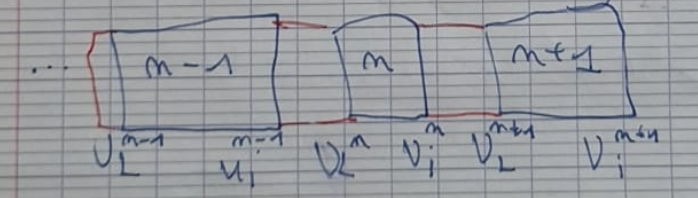
\includegraphics[scale=.5]{photo27.png}
		\end{minipage}
	\end{rmq}
	
	\newpage
	
	\underline{Linéarisation d'un EVP (\textit{Eigen Value Problem}) quadratique :}\\
	On peut résoudre un EVP quadratique de dimension $M$ : $\left(D_{RL}\frac1\lambda + (D_l+D_R)+D_{LR}\lambda\right)\Phi = 0$.\\
	Il s'agit d'un palindrome $\left(A\lambda^{-1} + \underset{B^t}B + A^t\lambda\right)$. Il admet $2M$ solutions.\\
	On note $(\lambda_i,\frac1{\lambda_i})$ les valeurs propres avec \begin{minipage}[t]{15cm}
		$\abs{\lambda_i}<1 \to$ ondes progressives\\
		$\abs{\frac1{\lambda_i}} > 1 \to$ ondes régressives
	\end{minipage}\\
	
	Pour résoudre cet EVP, dont la dimension dépend du nombre de DDL (ou particules), nous l'écrivons sous la forme :
	$\left(D_{RL} + (D_L+D_R)\lambda + D_{LR}\lambda^2\right)\Phi = 0$\\
	puis $\left(-D_{RL}-D_R\lambda\right)\Phi = \left(D_L\lambda + D_{LR}\lambda^2\right)\Phi$\\
	
	Ce qui s'écrit : $\underbrace{\begin{bNiceMatrix}[margin]
		 -D_{RL} & -D_R \\
		 0 & I
		 \CodeAfter
		 \SubMatrix[{1-1}{1-2}][extra-height=-.2cm]
		 \SubMatrix[{2-1}{2-2}][extra-height=-.2cm]
	\end{bNiceMatrix}}_N
	\begin{bmatrix}
		\Phi \\ \lambda\Phi
	\end{bmatrix} = \lambda \underbrace{\begin{bNiceMatrix}[margin]
		D_L & D_{LR} \\
		I & 0
		\CodeAfter
		\SubMatrix[{1-1}{1-2}][extra-height=-.17cm]
		\SubMatrix[{2-1}{2-2}][extra-height=-.17cm]
	\end{bNiceMatrix}}_{L}\underbrace{\begin{bmatrix}
	\Phi \\ \lambda\Phi
	\end{bmatrix}}_{\Psi}$\\
	
	L'EVP quadratique de dimension $M$ est désormais un EVP linéaire de dimension $2M$
	\[
	\left(N-\lambda L\right)\Psi = 0
	\]
	
	\noindent Lors d'application numériques on utilisera cette forme avec $\Big[\Gamma,\Psi\Big] = \text{eig}(N,L)$, \\
	puis on récupère $\overset{\cdot\cdot}\Phi = \overset{\cdot\cdot}\Psi \left[1:M\right]$\\
	Pour les systèmes de grande dimension ($M>100$) on peut régulariser le problème en introduisant un facteur $\rouge\sigma$.\\
	
	$\begin{bmatrix}
		-D_{RL} & -D_R \\
		0 & \rouge\sigma
	\end{bmatrix}\begin{bmatrix}
	\Phi \\ \lambda\Phi
	\end{bmatrix} = \begin{bmatrix}
	D_L & D_{LR} \\
	\rouge\sigma I & 0
	\end{bmatrix}\begin{bmatrix}
	\Phi \\ \lambda\Phi
	\end{bmatrix}$ où $\rouge\sigma$ est de l'ordre de $\mathbb D$.
	
	
\section{Dynamique des systèmes périodiques finis}
\subsection{Solutions en ondes d'une corde vibrante}
\begin{enumerate}[label=$\cdot$]
	\item On considère d'équation d'ondes dans le cas homogène scalaire.\\
$\begin{cases}
	\partial_t^2 U(t,x) -c^2\partial_x^2 U(t,x) = 0 \\
	U(t,x=a) = V_a(t)\\
	U(t,x=b) = V_b(t)
\end{cases}$ conditions aux limites/ déplacement imposé\\

$V_a$ et $V_b$ peuvent représenter des excitations imposés par un actionneur , ou des perturbations ou encore un encastrement.

	\item Appliquons une transformation de Fourier en temps :$U(t,x) = \dfrac1{\sqrt{2\pi}}\displaystyle\int_{-\infty}^{+\infty} U(\omega,x)e^{i\omega t}\mathrm d\omega$\\
	On a alors : $\begin{cases}
		\partial_x^2 U(\omega,x)+\left(\frac\omega c\right)^2U(\omega,x) = 0 \\
		U(\omega,a) = V_a(\omega)\\
		U(\omega,b) = V_b(\omega)
	\end{cases}$
	
	\item On suppose connu e nombre d'onde (i.e. $k(\omega)=\frac\omega c$), obtenu par une analyse de dispersion (Partie I).
\end{enumerate}
	
La solution générale de l'EDO harmonique est une superposition linéaire de deux solutions indépendanes : 
\[
U(\omega,x) = A^+(\omega)e^{-ik(\omega)x} + A^-(\omega)e^{ik(\omega)x}
\]
où $A^+$ et $A^-$ sont les amplitudes d'ondes (complexes), déterminées par les conditions aux limites.\\
La solution complexe (dont les déplacement sont la partie réelle) est donc :
\[
U(t,x) = \dfrac1{\sqrt{2\pi}}\displaystyle\int_{-\infty}^{+\infty}A^+(\omega)e^{i(\omega t-kx)}+A^-(\omega)e^{i(\omega t+ kx)}\mathrm d\omega
\]


\subsection{Généralisation à système Multi-ondes/Multi-DDL}

\subsubsection{Guide d'ondes uniforme vectoriel}

On suppose désormais le guide d'ondes \underline{vectoriel} (i.e. contenant $M$ DDL/atomes) par section.

\begin{ex}
	$\begin{cases}
		\text{- Poutre de Euler-Bernouilli}\\
		\text{- Cordes couplées}
	\end{cases}$
\end{ex}

Pour une onde (j) la décomposition de $\vec{U}(\omega,x)$ s'écrit :
\[
\vec U_j(\omega,x) = \vec\Phi^+(\omega)e^{-ikx}A^+(\omega) + \vec\Phi^-(\omega)e^{ikx}A^-(\omega)
\]	
où $\vec\Phi = \begin{bmatrix}
	\Phi^{(1)}\\\vdots\\\Phi^{(M)}
\end{bmatrix}$ est un vecteur de dimension $M$, vecteur propre de l'équation de dispersion, normalisé, et analogue à un mode propre.\\
On note $\Phi^+, A^+$ les ondes associées à $Im(k) < 0$ (progressives)\\
On note $\Phi^-, A^-$ les ondes associées à $Im(k) > 0$ (régressive).\\
Les $\Phi$ décrivent la "polarisation" de l'onde ou les déplacements des $M$ composantes sous l'effet de la propagation de l'onde.

\subsubsection{Cependant une décomposition de $\vec U$ sur une seule onde serait incomplète sous l'effet de la propagations de l'onde}

Donc la solution complète est une superposition des $M$ ondes :

\[
\vec U(\omega, x) = \displaystyle\sum_{j=1}^M \vec\Phi_j^+ e^{-ik_j x}A_j^+ + \vec\Phi_j^- e^{ik_j x}A_j^-
\]

sous la forme plus compacte :

\[
\fbox{$\vec U(\omega,x) = \underline{\underline{\Phi^+}} \underline{\Gamma^+}(x) \underline{a^+} + \underline{\underline{\Phi^-}} \underline{\Gamma^-}(x) \underline{a^-}$}
\]
	
où $\underline{\underline{\Phi^\pm}} = \left[\underline{\Phi_1^\pm},\cdots,\underline{\Phi_M^\pm}\right]$\\
$\underline{\underline{\Gamma^\pm}}(x) = diag\left(e^{\mp ik_1 x},\cdots,e^{\mp ik_M x}\right)$ et $\underline{a}^\pm = \begin{bmatrix}
	A_1^\pm \\ \vdots \\ A_M^\pm
\end{bmatrix}$


\includegraphics[scale=.5]{photo29.png}

De même que pour le cas scalaire, les ampliudes $\underline{a}^+$n et $\underline{a}^-$ ($2M$ inconnues) sp,t déterminées à partir des CL.\\
Dans le cas temporel/transitoire, la solution devient :
\[
\vec U(t,x) = \dfrac1{\sqrt{2\pi}}\displaystyle\int_\R \left[\Phi^+\Gamma^+a^+ +\Phi^-\Gamma^- a^-\right]e^{i\omega t}\mathrm d\omega
\]

\subsection{Décomposition en ondes de Bloch pour un guide périodique, scalaire, fini}

\subsubsection{Considérons la chaîne monoatomique (équiv. à une corde avec masses localisés périodique)}

Eq. (connue) du système est : $\begin{cases}
	m\partial_t^2 U_n = \beta\left(U_{n+1}+U_{n-1} - 2U_n\right)\\
	U_0(t) = V_0(t) \text{ et } U_N(t) = V_N(t)
\end{cases}$
	

\includegraphics[scale=.5]{photo30.png}

En analyse fréquentielle (régime stationnaire, ou après transformée de Fourier) on a :\\
$\begin{cases}
	U_{n+1} + \left(\Omega^2 -2\right)U_n + U_{n-1} = 0 \\
	U_0 = V_0\\
	U_N = V_N
\end{cases}$ $\forall n  \in [\![1,N-1]\!]$ où $\Omega = \frac\omega{\omega_0}$ et $\omega_0 = \sqrt{\frac\beta m}$\\

\subsubsection{Nous supposons que l'étude de dispersion effectuée dans le guide, c.a.d. nous connaissons $k(\omega)$, et donc $\lambda(\omega)$, $\forall \omega$}
	
La solution générale de l'Eq. aux différences finies/harmoniques est la superpositions de deux solutions indépendantes ($+$ et $-$) :
\[
U_n(\omega) = \lambda^n A^+(\omega) + \lambda^{-n}A^-(\omega) \text{ où $ A^+$ et $A^-$ sont les amplitudes complexes (inconnues)}
\]

Pour conserver les puissances de $\lambda$ positives, on choisit $A^- = \lambda^N A^-$.\\
ce qui donne : $\begin{aligned}[t]
	U_n &= \lambda^n A^+ + \lambda^{N-h} A^- \\
	&= e^{-iknd}A^+ + e^{ik(N-n)d} A^-
\end{aligned}$\\
La solution temporelle devient : $U_n(t) = \dfrac1{\sqrt{2\pi}}\displaystyle\int_\R e^{i(\omega t - knd)} A^+ + e^{i(\omega t - k(N-n)d)}A^- \mathrm d\omega$.\\



\subsection{Décomposition en ondes de Bloch dans une structure périodique finie}

\subsubsection{Rappel}
 L'équation d'équilibre donne l'EDO suivante :
 
 \[
 D_{RL} U_{n+1} + (D_L+D_R)U_n + D_{LR} U_{n+1} = 0
 \]
	
La relation de dispersion $\left(\frac1\lambda D_{RL} + (D_l+D_R) + \lambda D_{LR}\right)\Phi_{M,1} = 0$\\

donne $2M$ solutions : $\begin{aligned}[t]
	\to M \text{progressives ($\abs\lambda <1$) notées ($\lambda_j,\vec\Phi_j^+$)}\\
	\to M \text{ régressives ($\abs\lambda > 1$) notées ($\frac1\lambda, \vec\Phi_j^-$)}
\end{aligned}$\\

Pour une seule onde, la décomposition s'effectue de façon similaire au cas uniforme vectoriel :

 \[\vec U_n^{(j)} = \vec\Phi_j^+ e^{-ik_j dn}A_j^+ + \vec\Phi_j^- e^{-ik_jd(N-n)} A_j^- \]
 
où encore :

\[\vec U_n^{(j)} = \vec\Phi_j^+ \lambda_j^n A_j^+ + \vec\Phi_j^-\lambda_j^{N-n}A_j^-\]
	
	\subsubsection{La solution générale d'un système multi-modal fini est donc une superposition des $M$ ondes qui s'écrit :}
	
	\[
	U_n(\omega) = \displaystyle\sum_{j=1}^M \vec\Phi_j^+ \lambda_j^nA_j^+ + \vec\Phi_j^-\lambda_j^{N-n}A_j^-
	\]
	
	ou encore : 
	
	\begin{center}
		\enc[6cm]{red}{$U_n =\underline{\underline{\Phi}}^+\underline{\underline{\Lambda}}^n\underline{a}^++\underline{\underline{\Phi}}^-\underline{\underline{\Lambda}}^{N-n}\underline{a}^-$}
	\end{center}
	
	où $\Phi^\pm = \left[\underline{\Phi}_1^\pm,\cdots,\underline{\Phi}_M^\pm\right]$; $\underline{a}^\pm = \begin{bmatrix}
		A_1^\pm \\  \vdots \\ A_M^\pm
	\end{bmatrix}$ et $a_i^\pm = A_i^\pm$\\
	
	$\Lambda = \begin{bmatrix}
		\lambda_1 \\
		& \ddots \\
		&&\lambda_M
	\end{bmatrix}$\\
	
	En régime transitoire :
	
	$\underline{U}_n(t) = \frac1{\sqrt{2\pi}}\displaystyle\int_{-\infty}^{+\infty} \sum_{j=1}^M \Phi_j^+A_j^+e^{i(\omega t - k_j dn)} + \Phi_j^- e^{i(\omega t -k_jd(N-n))}\mathrm d\omega$\\
	
	où $\underline{U}$ est un vecteur à $M$ composantes et où les $2M$ inconnues ($\underline a^+,\underline a^-$) sont déterminées par les conditions aux limites.\\
	
	\underline{Remarques :}\\
	\begin{enumerate}[label = $\star$]
		\item Cette décomposition prend la forme d'une projection de $\vec U_n$ sur $\begin{bmatrix}
			\underline a^+ \\
			\underline a^-
		\end{bmatrix}$ c'est-à-dire $\underline{u} = \underline{\underline{P}} \hspace{.08cm}\underline{a}$
		
		\item \begin{minipage}{5cm}
			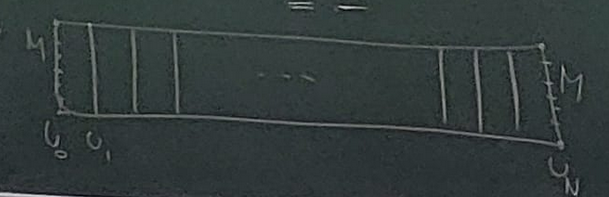
\includegraphics[scale=.2]{photo32.png} 
		\end{minipage}\begin{minipage}{15cm}
		\begin{enumerate}[label=$\star$]
			\item ce système possède $(N+1)M$ inconnues $U_n^{(j)}$, $n \in [\![0,N]\!]$, $j \in [\![1,M]\!]$
			
			\item En base ondulatoire, le système a $2M$ ($\underline a^-,\underline a^-$) inconnues
		\end{enumerate}
		\end{minipage}
	\end{enumerate}
	
	\underline{Synthèse :}
	
	\begin{NiceTabular}{c|c|c}
	\toprule
	& Uniforme $U(x)$ & Périodique \\
	\midrule
	1DDL - 1 onde & $U(x) = e^{-ikx}A^++e^{-ik(L-x)}A^-$ & $U_n = \lambda^n A^+ \lambda^N-nA^-$\\
	\midrule
	$M$ DDL - $M$ onde & $\vec U(x) = \vec\Phi^+ e^{-ikx}A^+ + \vec\Phi^- e^{-ik(L-x)}A^-$ & $\vec U_n = \vec\phi^+\lambda^n A^+ + \vec\phi^-\lambda^{N-n}A^-$ \\
	\midrule
	\Block{}{1 DDL - $M$ ondes\\ forme développée} & $U(x) = \displaystyle\sum_{j=1}^M e^{-ik_j x} A_j^+ + e^{-ik_j (L-x)}A_j^-$ & $U_n = \displaystyle\sum_{j=1}^M \lambda_j^nA_j^+ + \lambda_j^{N-n}A_j^-$\\
	\midrule
	\Block{}{$M$ DDL - $M$ ondes\\ forme développée} & $\vec U(x) = \displaystyle\sum_{j=1}^M \vec\Phi_j^+ e^{-ik_j x} A_j^+ + \vec\Phi_j^- e^{-ik_j(L-x)}A_j^-$ & $\vec U_n = \displaystyle \sum_{j=1}^M \vec\phi_j^+\lambda_j^n A_j^+ + \vec\phi_j^- \lambda_j^{N-n}A_j^-$\\	
	\midrule
	\Block{}{$M$ DDL - M ondes \\ forme compacte \\ (matricielle)} & $\vec U(x) = \underline{\underline{\Phi}}^+\underline{\underline{\Gamma}}(x)\underline{a}^+ + \underline{\underline{\Phi}}^-\underline{\underline{\Gamma}}(L-x)\underline{a}^-$ & $U_n =\underline{\underline{\Phi}}^+\underline{\underline{\Lambda}}^n\underline{a}^++\underline{\underline{\Phi}}^-\underline{\underline{\Lambda}}^{N-n}\underline{a}^-$\\
	\bottomrule
	\end{NiceTabular}
	
	\begin{enumerate}[label=$\star$]
		\item $k, \lambda$ sont solutions (valeurs propres) d'une relation de dispersion
		
		\item  $\Phi^+, \Phi^-$ sont vecteurs propres
		
		\item  Les amplitudes $a^+, a^-$ sont les nouvelles inconnues, calculées à partir des C.L. (ex. $\begin{cases}
			x = 0 \\ x = L
		\end{cases} $ ou $\begin{cases}
		n= 0 \\ n= N
		\end{cases}$)
		
		\item  Dans le cas d'une analyse harmonique en $\omega$ (régime stationnaire) , seul $U(\omega)$ est à calculer (mono-fréquence)
		
		\item Dans le cas transitoire, on doit calculer $U(\omega)$ pour toutes les fréquences de la transformée de Fourier, puis intégrer les $U_n(\omega)$ pour obtenir $U_n(t)$.
		
		\item  \begin{minipage}[t]{18.5cm}
			Des divergences peuvent être observées aux résonances, si le modèle 'est pas amorti (i.e. $\mathbb K - \omega^2 \mathbb  M$ avec $\mathbb M$ et $\mathbb K$ réels).
		Modèle dispersif classique en dynamique $\mathbb K^\star = \mathbb K (1+i\eta)$, où $\eta$ : facteur de perte $\sim 1/n$
		\end{minipage}
	\end{enumerate}
	
\newpage
	
\subsection{Écriture des conditions aux limites et assemblage de structures périodiques \underline{finies}}


\subsubsection{Chaîne mono-atomique}
	
	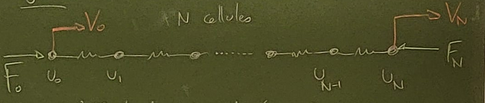
\includegraphics[scale=.5]{photo33.png}
	
	On considère une chaîne monoatomique finie constituée de $N$ cellules ($N+1$) atomes, en régime stationnaire. Le système d'équation s'écrit :
	
	\[
	\begin{bmatrix}
		k-\omega^2 m & -k \\
		-k & \cdots \\\\\\
		& &  - k & k-\omega^2 & -k \\\\\\
		& & & & \cdots & -k \\
		& & & & -k & k-\omega^2 m
	\end{bmatrix}\begin{bmatrix}
	U_0 \\  U_1 \\ \vdots \\ U_{n-1}\\U_n \\ U_{n+1} \\\vdots\\U_{N-1}\\U_N
	\end{bmatrix} = \begin{bmatrix}
	f_0 \\ \\ 
	\vdots\\ \\
	\vdots\\ \\
	\vdots\\ \\
	f_N
	\end{bmatrix}
	\]
	
	Dans l'exercice précédent, nous avions imposé $U_0$ et $U_N$ : l'écriture des C.L.\\
	Que se passe-t-il lorsque l'on ne connaît pas les déplacement $U_0$, mais la force extérieur (ex. $F_0$) ?\\
	
	Si \underline{$S_0 =F_0$} est imposé, alors $U_0$ est inconnue. Développons la 1ère ligne du système :
	\[
	(k-\omega^2 m)U_0-kU_1 = F_0
	\] 
	or nous connaissons également $U_1$ grâce à la décomposition en ondes de Bloch : $\forall n, U_n = \lambda^n A^+ + \lambda^{N-n}A^- \implies\begin{cases}
		U_0 = A^+ + \lambda A^- \\
		U_1 = \lambda A^+ +\lambda^{N-1}A^-
	\end{cases}$\\
	cela donne : $(k-\omega^2 m)(A^+ + \lambda^N A^-) - k(\lambda A^+ + \lambda^{N-n}A^-) = F_0$\\
	
	\[
	\left[k-\omega^2 m-k\lambda\right]A^+ + \left[(k-\omega^2 m)\lambda^N-k\lambda^{N-1}\right]A^- = F_0
	\]
	
	Si \underline{$S_N = F_N$} est imposée, on développe la $N^{ième}$ ligne (équilibre des forces en $U_N$) :\\
	$-kU_{N-1}+(k-\omega^2 m)U_N = F_N$, on décompose $\begin{cases}
		U_{N-1} = \lambda^{N-1}A^+ + \lambda A^-\\
		U_N = \lambda^N A^+ + A^-
	\end{cases}$\\
	
	ceci donne :
	
	\[
	\left[-k\lambda^{N-1}+(k-\omega^2 m)\lambda^N\right]A^+ + \left[-k\lambda+(k-\omega^2 m)\right]A^- = F_N
	\]
	
	Pour trouver $A^+$ et $A^-$ on doit donc résoudre le système :
	
	\[
	\underbrace{\begin{bmatrix}
		k-\omega^2 m - k\lambda & (k-\omega^2m)\lambda^N-k\lambda^{N-1} \\
		(k-\omega^2m)\lambda^N - k \lambda^{N-1} & (k-\omega^2 m)-k\lambda
	\end{bmatrix}}_{H(\lambda,\omega)}\begin{bmatrix}
	A^+ \\ A^-
	\end{bmatrix} = \begin{bmatrix}
	F_0 \\ A_N
	\end{bmatrix} \implies \begin{bmatrix}
	A^+ \\ A^-
	\end{bmatrix} = H(\lambda,\omega)^{-1}\begin{bmatrix}
	F_0 \\ F_N
	\end{bmatrix}
	\]
	
	
	\subsubsection{Condition aux limites ($U,F$) dans le cas général}
	
	On considère la structure périodique finie, constituée par un assemblage de cellules périodiques identiques décrites par la raideur dynamique $\mathbb D= \begin{bmatrix}
		D_L & D_{LR} \\
		D_{RL} & D_R
	\end{bmatrix}$
	
	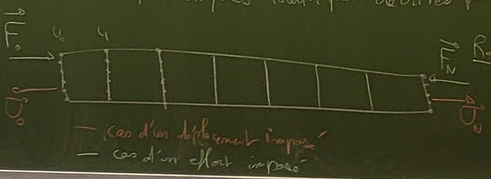
\includegraphics[scale=.5]{photo34.png}
	
	\begin{rmq}
		Ici on utilise une matrice sans DLL internes ($U_I = \{\}$), où bien une matrice où les DDL internes sont condensés sur $U_L, U_R$
	\end{rmq}
	
	Le système global s'écrit alors :
	
	\[
	\begin{bmatrix}
		D_L & D_{LR} \\
		D_{RL} & D_R+D_L & D_{LR} \\
		& D_{RL} & \ddots & \ddots \\
		& & \ddots & \ddots & \ddots \\
		& & & D_{RL} & D_L+D_R & D_{LR} \\
		& & & & D_{RL} & D_R
	\end{bmatrix}\begin{bmatrix}
	U_0 \\
	U_1 \\ \\
	\vdots \\ 
	U_{N-1} \\
	U_N
	\end{bmatrix} = \begin{bmatrix}
	f_0 \\
	0 \\ \\
	\vdots \\ 
	0 \\
	f_N
	\end{bmatrix} \iff \mathbb D_{global}U_{global} = F_{global}
	\]
	
	\begin{enumerate}
		\item Cas \underline{$U_0-U_N$ imposés}. On a donc $\begin{cases}
			u_0 = U_0\\
			u_N = U_N
		\end{cases}$ connus. On ignore les notations $\underline{\cdot}$ et $\underline{\underline{\cdot}}$\\
		La décomposition en ondes de Bloch est, dans le cas vectoriel ($M$ DDL), multimodal ($M$ ondes), $\forall n \in [\![0,N]\!], \underline{U}_n = \underline{\underline{\Phi}}^+\underline{\underline{\Lambda}}^n\underline{a}^+ + \underline{\underline{\Phi}}^-\underline{\underline{\Lambda}}^{N-n}\underline{a}^-$\\
		ceci donne : $\begin{cases}
			u_0 = \Phi^+ a^+ + \Phi^-\Lambda^N a^- = U_0 \\
			u_N = \Phi^+ \Lambda^N a^+ + \Phi^- a^- = U_n
		\end{cases}\iff \underbrace{\begin{bmatrix}
		\Phi^+ & \Phi \Lambda^N \\
		\Phi^+\Lambda^N & \Phi^+
		\end{bmatrix}}_H\underbrace{\begin{bmatrix}
		a^+ \\ a^-
		\end{bmatrix}}_{a} = \underbrace{\begin{bmatrix}
		U_0 \\ U_N
		\end{bmatrix}}_{U}$\\
	
		Donc $\begin{bmatrix}
			a^+ \\ a^-
		\end{bmatrix} = H^{-1}\begin{bmatrix}
		U_0 \\ U_N
		\end{bmatrix}$ est la solution, qui nous donne ensuite $U_n$ pour tout $n \in \N$.
		
		\newpage
		
		\item \underline{Cas $F_0 - F_N$ imposés}
		
		Lorsque les efforts extérieurs sont appliqués aux extrémités $n=0$ et $n=N$, on écrit l'équilibre des forces en $n=0$ et $n=N$, ce qui revient à développer les $1^{ère}$ et $N^{ième}$ lignes du système $D_yU_y = F_y$, c'est-à-dire : $\begin{cases}
			D_L U_0 + D_{LR} U_1 = F_0\\
			D_{RL}U_{N-1} + D_RU_N=F_N
		\end{cases}$ ou $\begin{cases}
		U_1 = \Phi^+\Lambda a^+ + \Phi^-\Lambda^{N-1}a^- \\
		U_{N-1} = \Phi^+\Lambda^{N-1}a^+ + \Phi^-\Lambda a^-
		\end{cases}$\\
		$\begin{cases}
			D_L(\Phi^+a^++\Phi^-\Lambda^Na^-)+D_{LR}(\Phi^+\Lambda a^+ + \Phi^-\Lambda^{N-1}a^-) = F_0\\
			D_{RL}(\Phi^+\Lambda^{N-1}a^+ + \Phi^-\Lambda a^-) + D_R(\Phi^+\Lambda^N a^++\Phi^-a^-) = F_N
		\end{cases}$\\
		Sous forme matricielle, cela donne :\\
		\enc[13.5cm]{red}{$\begin{bmatrix}
				D_L\Phi^+ + D_{LR}\Phi^+\Lambda & D_L\Phi^-\Lambda^N + D_{LR}\Phi^-\Lambda^{N-1} \\
				D_{RL}\Phi^+ \Lambda^{N-1} + D_R\Phi^+\Lambda^N & D_{RL}\Phi^-\Lambda + D_R\Phi^-
			\end{bmatrix}\begin{bmatrix}
			a^+ \\ a^-
			\end{bmatrix} = \begin{bmatrix}
			F_0 \\ F_N
			\end{bmatrix}$}
	\end{enumerate}
	
	
	
	
	
	
	
	
	
	
	
	
	
	
	
	
	
	
	
	
	
	
	
	
	
	
	
	
	
	
	
	
	
	
	
	
	
	
	
	
	
	
	
	
	
	
	
	
	
	
	
	
	
	
	
	
	
	
	
	
	
	
	
	
	
	
	\newpage
	
	\section{TD}
	
	\subsection{système périodique : Introduction (section 1 - 2.2)}
	
	\begin{exo}[Système périodique et résonance locale]$ $\\
		\textbf{\underline{Rappel démarche :}}
		
		\vspace{-.5cm}
		
		\begin{minipage}[t]{18.5cm}
			\begin{enumerate}
				\item Identifier la période (cellule périodique minimale du système)
				\item  Écrire les équations d'équilibre (opérateur $\m L U(x,t) = 0$) pour chaque degré de liberté
				\item Invoquer la stationnarité ($U(x,t) \to u(x,\omega)$) puis le principe de Floquet-Bloch :
				\[(u_{n+1},u_{n-1},\ldots, \to \left(\lambda,\frac{1}{\lambda}\right)u_n) \text{ où } u_n(t) = u_0 e^{i(nka-\omega t)}\]
				\item Équation l'équation de dispersion (ou système $\to \det = 0$) liant $\omega$ et $\lambda$.
				\item Résoudre $((i)$ $\omega(k),$ (ii) $k(\omega))$
				\item Interpréter les solutions $\left(\left[\begin{minipage}{2.5cm}
					\text{propagatives}\\\text{évanescentes}
				\end{minipage}\right] et \left[\begin{minipage}{3cm}
					\text{progressive + }$x$\\\text{régressive + }$x$
				\end{minipage}\right]\right)$ et tracer.
			\end{enumerate}
		\end{minipage}
		
		
		
\includegraphics[scale=.5]{photo8.png}
		
		On produit des bandes interdites sous forme "additive".\\
		Si $m_2\to 0$, on doit retrouver la chaîne mono-atomique.
	\end{exo}
	
	\begin{sol}$ $
		
		\vspace{-.5cm}
		
		\begin{enumerate}
			\item On identifie la période : 
\includegraphics[scale=.2]{photo9.png} 
			
			\item On écrit les équations d'équilibre :
			\[\begin{aligned}
				\text{(1) }&m_1\dfrac{d^2 U_n}{dt^2} &=& -\beta_1(U_n-U_{n+1})-\beta_1(U_n-U_{n-1}) - \beta_2(U_n-V_n)\\\\
				\text{(1) }&m_1\dfrac{d^2 U_n}{dt^2} &= &\beta_1(U_{n+1}-2U_n+U_{n-1}) + \beta_2(V_n-U_n)\\\\
				\text{(2) }& m_2\dfrac{d^2 V_n}{dt^2} &= &\beta_2(U_n-V_n)
			\end{aligned}\]
			
			\item On considère le régime stationnaire et le principe de Floquet-Bloch : $U_n = U_0\lambda^n e^{i\omega t}$ et $V_n = V_0 \lambda^n e^{i\omega t}$. Et on réécrit les 2 équations :
			\[\begin{aligned}
				\text{(1) } -m_1\omega^2 U_0 &= \beta_1(\lambda U_0 - 2U_0 + \frac{1}{\lambda}U_0)+\beta_2(V_0-U_0)\\
				\text{(2) } -m_2 \omega^2 V_0 &= \beta_2(U_0-V_0)
			\end{aligned} \]
			
			Puis, on divise $(i)$ par $m_i$ :
			\[\begin{aligned}
				-\omega^2 U_0 &= \frac{\beta_1}{m_1}(\lambda U_0 - 2U_0 + \frac{1}{\lambda}U_0)+\frac{\beta_2}{\beta_1}\frac{\beta_1}{m_1}(V_0-U_0)\\
				-\omega^2 V_0 &= \beta_2/m_2(U_0-V_0)
			\end{aligned} \]
			
			\begin{minipage}[t]{18cm}
				On regroupe selon $U_0$ et $V_0$ et on utilise les notations suivantes : $\omega_1=\sqrt{\frac{\beta_1}{m_1}}$, $\omega_2 = \sqrt{\frac{\beta_2}{\beta_1m_2}}$ et $r = \frac{\beta_2}{\beta_1}$  :
			\end{minipage}
			\[ \begin{aligned}
				(\omega^2 + \omega_1^2(\lambda+\frac{1}{\lambda}-2)-r\omega_1^2)U_0&+&r\omega_1^2 V_0&=0\\
				\omega_2^2 U_0&+&(\omega^2-\omega_2^2)V_0 &=0
			\end{aligned} \]
			
			
			On pose : $A = \left[\begin{matrix}
				\omega^2 + \omega_1^2(\lambda+\frac{1}{\lambda}-2-r) & r\omega_1^2\\
				\omega_2^2 & \omega^2-\omega_2^2
			\end{matrix}\right]$ et on a ainsi : $AX = 0$ où $X = \left[\begin{matrix}
				U_0\\ V_0
			\end{matrix}\right]$.
			
			Regardons le déterminant pour trouver une condition nécessaire et suffisante pour trouver des solutions non trivial :
			\[\begin{aligned}
				&\det A = 0\\
				\iff&\left[\omega^2 + \omega_1^2(\lambda+\frac{1}{\lambda}-2-r)\right]\times (\omega^2-\omega_2^2) - r\omega_1^2\omega_2^2 =0\\
				\iff & \omega^4 + \omega^2 \left[\omega_1^2(\lambda+\frac{1}{\lambda}-2-r)-\omega_2^2\right]-w_1^2w_2^2\left[r+\lambda+\frac{1}{\lambda}-2-r\right] = 0\\
				\iff&\omega^4 + \omega^2 \left[\omega_1^2(\lambda+\frac{1}{\lambda}-2-r)-\omega_2^2\right]-w_1^2w_2^2\left[\lambda+\frac{1}{\lambda}-2\right] = 0\\
				\iff&\omega^4 + \omega^2 \left[\omega_1^2\left(2\left[cos(ka)-1\right]-r\right)-\omega_2^2\right]-2w_1^2w_2^2\left(\cos(ka)-1\right) = 0
			\end{aligned}\]
			
			Puis on regarde le discriminant :
			\[\begin{aligned}
				\Delta &=\left[\omega_1^2\left(2\left[cos(ka)-1\right]-r\right)-\omega_2^2\right]^2+8w_1^2w_2^2\left(\cos(ka)-1\right)\\
				&=\left[2\omega_1^2\left[cos(ka)-1\right]-\omega_2^2-\omega_1^2 r\right]^2+8w_1^2w_2^2\left(\cos(ka)-1\right)\\
				&=\left[2\omega_1^2\left[cos(ka)-1\right]-\omega_2^2\right]^2+\omega_1^4 r^2+8w_1^2w_2^2\left(\cos(ka)-1\right)\\
				&=\cdots\\
				\Delta&>0
			\end{aligned}\]
		\end{enumerate}
		
		\newpage
		
		\textbf{\underline{Tracé des solutions :}} Il y a 2 cas : $\begin{cases}
			\omega_2 <2\omega_1\\
			\omega_2 = 2 \omega_1\\
			\omega_2 > 2\omega_1
		\end{cases}$ :
		
		
\includegraphics[scale=.5]{photo10.png}
		
		Pour calculer le $k$ complexe dans la bande interdite, on doit résoudre $k(\omega)$. L'équation de dispersion peut se réécrire en notant : $\Omega_1^2 = \frac{\omega^2}{\omega_1^2}$ et $\Omega_2^2 = \frac{\omega^2}{\omega_2^2}$ :
		
		\[\implies  \lambda^2 + \left[\Omega_1^2+r\dfrac{\Omega_2^2}{1-\Omega_2^2}-2\right]+1 = 0\]
		
		\[k(\omega) = \frac{i}{a}\log\left[1-\frac{\Omega_1^2}{2}-\frac{r}{2}\frac{\Omega_2}{1-\Omega_2^2} \pm \sqrt{\left(\Omega_1^2+\frac{r\Omega_2^2}{1-\Omega_2^2}\right)\left(\Omega_1^2+\frac{r\Omega_2^2}{1-\Omega_2^2}-4\right)}\right]\]
	\end{sol}
	
	\subsection{Condensation dynamique (section 2.3 - 2.4)}
	\begin{exo}[Formulation matricielle]
		\begin{minipage}[t]{15cm}
			Appliquer à la chaîne monoatomique, en considérant la cellule périodique :
		\end{minipage}
		
		
\includegraphics[scale=.5]{photo18.png}.
		
		\begin{enumerate}
			\item Déterminer les matrices de masses et raideurs :
			\[
			\mathbb{K}_e, \mathbb{M}_e \text{ puis } \mathbb{D} = \left[\begin{matrix}
				D_L & D_{LR}\\
				D_{RL} & D_R
			\end{matrix}\right]
			\]
			
			\item Ecrire la matrice globale du système infini.
			
			\item Appliquer le principe de Floquet-Bloch ($U_{n+1}$ et $U_{n-1}$ en fonction de $U_n$ et $\lambda$) et en déduire l'équation de dispersion.
		\end{enumerate}
	\end{exo}
	
	\begin{sol}$ $\\
		\begin{enumerate}
			\item $\mathbb{M}_e = \left[\begin{matrix}
				\frac{m}{2} & 0 \\
				0 & \frac{m}{2}
			\end{matrix}\right]$ et $\mathbb{K}_e=\left[\begin{matrix}
				K & -K \\
				-K & K
			\end{matrix}\right]$\\
			$\mathbb{D} = k_e-\omega^2\mathbb{M}_e = \left[\begin{matrix}
				k-\omega^2\frac{m}{2} & -k \\
				-k & k-\omega^2\frac{m}{2}
			\end{matrix}\right] = \left[\begin{matrix}
				D_L & D_{LR} \\
				D_{RL} & D_R
			\end{matrix}\right]$
			
			\item $\left[\begin{matrix}
				\ddots & \ddots & \ddots \\
				& -K & 2K-\omega^2m & -K \\
				& & \ddots & \ddots & \ddots 
			\end{matrix}\right]\left[\begin{matrix}
				\vdots \\ U_{n-1} \\ U_n \\ U_{n+1} \\ \vdots
			\end{matrix}\right] = \left[\begin{matrix}
				\vdots \\
				0 \\
				\vdots
			\end{matrix}\right]$
			
			\item \begin{minipage}[t]{18.5cm}
				Floquet-Bloch donne $\begin{cases}
					U_{n+1} = \lambda U_n \\
					U_{n-1} = \frac{1}{\lambda} U_n
				\end{cases}$ et $-KU_{n-1} + (2K-\omega^2n)U_n-KU_{n+1} = 0$
			\end{minipage}
			
			On en déduit l'équation de dispersion des ondes : 
			\[
			\left(-K\frac{1}{\lambda} + (2K-\omega^2m)-K\lambda\right)U_n = 0
			\]
			
			\begin{minipage}[t]{15cm}
				$\div(-K) \implies \left(\lambda + \omega^2\frac{m}{K} -2+\frac{1}{\lambda}\right)U_n = 0 \to $ Équation de dispersion
			\end{minipage}
			
			\begin{minipage}[t]{15cm}
				La forme $D_{RL}U_{n-1}+(D_L+D_R)U_n+D_{LR}U_{n+1} = 0$ est générale (elle s'applique à toute cellule périodique décrite par une raideur dynamique $\mathbb{D} = \left[\begin{matrix}
					D_L & D_{LR} \\
					D_{RL} & D_R
				\end{matrix}\right]$)
			\end{minipage}
			
			\enc{red}{La relation de dispersion est alors :
				
				\[
				\left(\frac{1}{\lambda} D_{RL} + (D_L+D_R)+D_{LR}\lambda\right)\overset{\textbf{..}}{U_n} = 0_{p,1} \text{ (1)}
				\]
			}
			
			\textbf{Note :} \begin{minipage}[t]{15cm}
				C'est un problème aux valeurs propres de dimension notée $p$, polynomiak, d'ordre 2. Il admet donc (en général) $2p$ solutions :
				\begin{enumerate}
					\item[$p$] solutions où $\abs{\lambda} < 1$ (progressives)
					\item[$p$] soltuions où $\abs{\lambda} > 1$ (régressives)
				\end{enumerate}
			\end{minipage}
		\end{enumerate}
	\end{sol}
	
	\newpage
	
	\begin{exo}[Suite de l'exercice précédent] $ $\\
		Écrire (1) sous la forme $\omega(k)$ c'est-à-dire : $(A-\omega^2B)\Phi = 0$.
	\end{exo}
	\begin{sol}
		\[\begin{aligned}
			\left(\frac{1}{\lambda}D_{RL}+(D_L+D_R)+\lambda D_{LR}\right)U_n = 0 \\
			\left[\frac{1}{\lambda}(K_{RL}-\omega^2M_{RL})+(K_L-\omega^2M_L)+(K_L-\omega^2M_L+K_R-\omega^2M_R)+\lambda(K_{LR}-\omega^2M_{LR})\right]U_n = 0\\
			\left(\underbrace{\left[\frac{1}{\lambda}K_{RL}+K_L+K_R+\lambda K_{LR}\right]}_{\overset{\sim}{K}(\lambda)}-\omega^2\underbrace{\left[\frac{1}{\lambda}M_{RL}+M_L+M_R+\lambda M_{LR}\right]}_{\overset{\sim}{M}(\lambda)}\right)U_n = 0
		\end{aligned}\]
		
		\begin{minipage}[t]{18cm}
			Le problème aux VP devient : \enc[5.5cm]{red}{$\left[\overset{\sim}{K}(\lambda) - \omega^2\overset{\sim}{M}(\lambda)\right]U_n = 0$} (2) forme $\omega(\lambda)$
		\end{minipage}
		
		En pratique : \begin{minipage}[t]{15cm}
			
			\vspace{-.3cm}
			
			\begin{enumerate}
				\item donne des solutions complexes ($\lambda \in \C$) pour $\omega$ réel donné.
				\item donner des solutions réelles ($\omega \in \R^*$) pour $k$ réel donné ($k \to \lambda = e^{iak}$).
			\end{enumerate}
			Sa résolution s'apparente au calcul de modes propres/fréquences propres.
		\end{minipage}
	\end{sol}
	
	\begin{exo}[Exo type d'examen] $ $\\
		On considère la cellule périodique suivante :\\
		
		\begin{minipage}{6cm}
			
\includegraphics[scale=.5]{photo19.png}
		\end{minipage}\begin{minipage}{15cm}
			\begin{enumerate}
				\item Ecrire le système d'EDP en $U_n$ et $V_n$.
				\item En déduire l'équation de dispersion.
				\item Choisir une cellule périodique et écrire $\mathbb{K}_e$, $\mathbb{M}_e$ pour $\mathbb{D}$.
				\item Retrouver directement d'équation de dispersion (matricielle).
			\end{enumerate}
		\end{minipage}
	\end{exo}
	\begin{sol}
		$ $\\
		\begin{enumerate}
			\item $\begin{cases}
				m\dfrac{\partial^2 U_n}{\partial t^2} = -K(U_n-U_{n-1}) - K(U_n-U_{n-1}) - \beta(U_n-V_n)\\\\
				m\dfrac{\partial^2 V_n}{\partial t^2} = -K(V_n-V_{n-1}) - K(V_n-V_{n+1}) - \beta (V_n-U_n)
			\end{cases}$
			
			\item \begin{minipage}[t]{18.5cm}
				$\begin{cases}
					U_n(t) = U_0e^{\i (nka-\omega t)}\\
					V_n(t) = V_0e^{\i(nka-\omega t)}
				\end{cases}$, où $a$ est la période.\\
				$\begin{cases}
					U_{n+1} = \lambda U_n \\
					U_{n-1} = \frac{1}{\lambda} U_n
				\end{cases}$ et $\begin{cases}
					V_{n+1} = \lambda V_n\\
					V_{n-1} = \frac{1}{\lambda} V_n
				\end{cases}$.\\
				On l'injecte dans l'équation : $\begin{cases}
					m\omega^2 U_n = K(U_n-\lambda U_n)+K(U_n-\frac{1}{\lambda}U_n) + \beta(U_n-V_n)\\
					m\omega^2V_n = K(V_n-\lambda V_n) + K(V_n-\frac{1}{\lambda}V_n) + \beta(U_n-V_n)\\
					m\omega^2V_n = K(V_n-\lambda V_n) + K(V_n-\frac{1}{\lambda}V_n)+\beta(V_n-U_n)
				\end{cases}$\\
				On pose $\omega_1 = \frac{K}{M}$ et $\omega_2 = \frac{\beta}{m}$, on a : $\begin{cases}
					(\omega^2-\omega_1(2-\lambda-\frac{1}{\lambda}) -\omega_2)U_n + \omega_2 V_n = 0\\
					(\omega^2-\omega_1(2-\lambda-\frac1\lambda))V_n-\omega_2U_n = 0
				\end{cases}$\\
				
				\[\fbox{$\left[\begin{matrix}
						\omega^2-\omega_1(2-\lambda-\frac{1}{\lambda})-\omega_2 & \omega_2\\
						\omega_2 & \omega^2-\omega_1(2-\lambda-\frac1\lambda) - \omega_2
					\end{matrix}\right]\left[\begin{matrix}
						U_n \\ V_n
					\end{matrix}\right] = \left[\begin{matrix}
						0 \\ 0
					\end{matrix}\right]$}\]
				
				\[\begin{aligned}
					\det(A) &= \left(\omega^2-\omega_1(2-\lambda-\frac{1}{\lambda})^2-\omega_2^2\right)^2 - \omega_2^2\\
					&= (\omega^2-\omega_1(2-\lambda-\frac1\lambda))(\omega^2-\omega_1(2-\lambda-\frac1\lambda)-2\omega_2)
				\end{aligned}\]
			\end{minipage}
			
			\item \begin{minipage}[t]{18.5cm}
				\begin{minipage}{5cm}
					
\includegraphics[scale=1]{photo20.png}
				\end{minipage}\begin{minipage}{15cm}
					$\mathbb{M}=\left[\begin{matrix}
						m & 0 & 0 & 0\\
						0 & m & 0 & 0 \\
						0 & 0 & 0 & 0 \\
						0 & 0 & 0 & 0
					\end{matrix}\right]$ et $\mathbb{K} = \left[\begin{matrix}
						K+\beta & -\beta & -K & 0 \\
						-\beta & k+\beta & 0 & -k \\
						-k & 0 & k & 0 \\
						0 & -k & 0 & k
					\end{matrix}\right]$
				\end{minipage}
				
				\underline{Rappel :} $\mathbb{M}\overset{\textbf{..}}{U}+\mathbb{K}U = 0 \implies \mathbb{D}U = 0$\\
				
				\[\mathbb{D} = \left[\begin{matrix}
					(K+\beta)-\omega^2m & -\beta & -K & 0 \\
					-\beta & (k+\beta)-\omega^2m & 0 & -K \\
					-K & 0 & K & 0 \\
					0 & -K & 0 & K
				\end{matrix}\right]\]
				
				$(D_{RL}\frac1\lambda + (D_L+D_R)+\lambda D_{LR})\vec{U}_L = 0$, où $\vec U_L = \left[\begin{matrix}
					U_L \\ V_L
				\end{matrix}\right]$
				
				\[
				\left(\frac1\lambda \left[\begin{matrix}
					-K & 0 \\
					0 & -K
				\end{matrix}\right]+\left[\begin{matrix}
					(K+\beta)-\omega^2 m + K & -\beta\\
					-\beta & (K+\beta)-\omega^2m+K
				\end{matrix}\right] + \lambda\left[\begin{matrix}
					-K & 0\\
					0 & -K
				\end{matrix}\right]\right)\vec U_L = \vec{0}
				\]
				
				\[
				\left[\begin{matrix}
					(K+\beta)-\omega^2m+K-(\frac1\lambda+\lambda)K & - \beta \\
					-\beta & (K+\beta)-\omega^2m + K-(\frac1\lambda + \lambda)K
				\end{matrix}\right]\left[\begin{matrix}
					U_L \\
					V_L
				\end{matrix}\right] = \left[\begin{matrix}
					0 \\ 0
				\end{matrix}\right]
				\]
			\end{minipage}	
		\end{enumerate}
	\end{sol}
	
	\begin{exo} \begin{minipage}[t]{15cm}
			On considère un système décrit pas les matrices dynamiques : 
		\end{minipage}
		\begin{minipage}{10cm}
			\[
			\left[\begin{matrix}
				D_L & D_{Li} & 0 \\
				D_{iL} & D_i & D_{iR} \\
				0 & D_{Ri} & D_R
			\end{matrix}\right]\left[\begin{matrix}
				U_L\\
				U_i\\
				U_R
			\end{matrix}\right] = \left[\begin{matrix}
				f_L \\ 0 \\ f_R
			\end{matrix}\right]
			\]
		\end{minipage}\begin{minipage}{5cm}
			
\includegraphics[scale=.5]{photo23.png}
		\end{minipage}
		
		Montrer que ce système peut s'écrire sous forme condensée :
		
		\begin{minipage}[t]{18cm}
			$\left[\begin{matrix}
			\overset\sim D_L & \overset\sim D_{LR} \\
			\overset\sim D_{RL} & \overset\sim D_R
		\end{matrix}\right]\left[\begin{matrix}
			U_L \\ U_R
		\end{matrix}\right] = \left[\begin{matrix}
			f_L \\
			f_R
		\end{matrix}\right]$, où on explicitera les $\overset\sim D_{ij}$, $i,j \in \{L,R\}$.
		\end{minipage}
	\end{exo}
	\begin{sol}
		on a : $D_{iL} U_L + D_iU_i + D_{iR}U_R = 0$.\\
		Si $D_i$ est inversible, on obtient  :
		\[
		U_i = D_i^{-1}\left(-D_{iL}U_L-D_{iR}U_R\right)
		\]
		$\begin{aligned}
			\to & D_LU_L - D_{Li}D_i^{-1}D_{iL}u_L-D_{Li}D_i^{-1}D_{iR}u_R = f_L\\
			& \iff -D_{Ri}D_i^{-1}D_{iL}U_L + (D_R-D_{Ri}D_i^{-1}D_{iR})u_R = f_L\\
			\to & -D_{Ri}D_i^{-1}D_{iL}u_L + (D_R-D_{Ri}D_i^{-1}D_{iR})u_R = f_R
		\end{aligned}$
		
		\[
		\left[\begin{matrix}
			\overbrace{D_L-D_{Li}D_i^{-1}D_{iL}}^{\overset\sim D_L} & \overbrace{-D_{Li}D_i^{-1}D_{iR}}^{\overset\sim D_{LR}} \\
			\underbrace{-D_{Ri}D_i^{-1}D_{iL}}_{\overset\sim D_{RL}} & \underbrace{-D_{Ri}D_i^{-1}D_{iL} + D_R}_{\overset\sim D_R}
		\end{matrix}\right] \left[\begin{matrix}
			U_L \\
			U_R
		\end{matrix}\right] = \left[\begin{matrix}
			f_L \\ f_R
		\end{matrix}\right]
		\]
		
		\textbf{\underline{Alternative}}
		
		\[
		\left[\begin{matrix}
			D_L & D_{Li} & 0 \\
			D_{iL} & D_i & D_{iR} \\
			0 & D_{Ri} & D_R
		\end{matrix}\right]\left[\begin{matrix}
			U_L \\ U_i \\ U_R
		\end{matrix}\right] = \left[\begin{matrix}
			f_L \\ 0 \\ f_R
		\end{matrix}\right] \iff \left[\begin{matrix}
			D_L & 0 & D_{Li} \\
			0 & D_R & D_{Ri} \\
			D_{iL} & D_{iR} & D_i
		\end{matrix}\right]\left[\begin{matrix}
			U_L \\ U_R \\ U_i
		\end{matrix}\right] = \left[\begin{matrix}
			f_L \\ f_R \\ 0
		\end{matrix}\right]
		\]
		
		$\implies$ On note $b := [L,R]$\\
		$\implies \left[\begin{matrix}
			D_b & D_{bi} \\
			D_{ib} D_i
		\end{matrix}\right]\left[\begin{matrix}
			U_b \\ U_i
		\end{matrix}\right] = \left[\begin{matrix}
			f_b \\ 0
		\end{matrix}\right]$\\
		On applique ensuite la condensation dynamique, i.e. :\\
		$ \overset\sim D_b = D_b - D_{bi}D_i^{-1}D_{ib}$ et $\overset\sim f_b = f_b-D_{bi}D_i^{-1}\overset{=0}{f_i} = f_b$
		
		\[
		\overset\sim D_b = \left[\begin{matrix}
			D_L & 0 \\
			0 & D_R
		\end{matrix}\right] - \left[\begin{matrix}
			D_{Li} \\ D_{Ri}
		\end{matrix}\right]D_i^{-1}\left[D_{iL}D_{iR}\right]
		\]
		
		$\begin{aligned}
			\overset\sim D_b &= \left[\begin{matrix}
				D_L & 0 \\
				0 & D_R
			\end{matrix}\right] - \left[\begin{matrix}
				D_{Li} \\
				D_{Ri}
			\end{matrix}\right]\left[\begin{matrix}
				D_i^{-1}D_{iL} & D_i^{-1}D_{iR}
			\end{matrix}\right]\\
			&=\left[\begin{matrix}
				D_L & 0 \\
				0 & D_R
			\end{matrix}\right] - \left[\begin{matrix}
				D_{Li} D_i^{-1}D_{iL} & D_{Li} D_i^{-1}D_{iR} \\
				D_{Ri}D_i^{-1}D_{iL} & D_{Ri}D_i^{-1}D_{iR}
			\end{matrix}\right]
		\end{aligned}
		$\\
		Donc $\overset\sim D_b = \left[\begin{matrix}
			D_L - D_uD_i^{-1}D_{iL} & -D_{Li}D_i^{-1}D_{iR} \\
			-D_{Ri}D_i^{-1} D_{iL} & D_R-D_{Ri}D_i^{-1}D_{iR}
		\end{matrix}\right]$.\\
		On vérifie la symétrie de $\overset\sim D$ :\\
		$\begin{cases}
			\overset\sim D_L ^T = \left(D_L-D_{Li}D_i^{-1}D_{iL}\right)^T = D_L^T -D_{iL}^TD_i^{-1 T}D_{Li}^T = D_L-D_{Li}D_i^{-1}D_{iL} = \overset\sim D_L\\
			\overset\sim D_{LR}^T = -(D_{Li}D_i^{-1}D_{iR})^T = D_{iR}^T(D_i^{-1})^TD_{Li}^T = -D_{Ri}D_i^{-1}D_{iL} = \overset\sim D_{RL}
		\end{cases}$
		
	\end{sol}
	
	\begin{exo}[application]
		\begin{minipage}[t]{12.5cm}
			appliquer cette méthode (celle de l'exercice précédent) pour écrire (sous forme matricielle) 'équation de dispersion de la chaîne à résonances locales :\\
			
			
\includegraphics[scale=.5]{photo24.png}
		\end{minipage}		
		
		\begin{enumerate}
			\item Ecrire $\mathbb K, \mathbb M$ puis $\mathbb D$ pour une cellule périodique "seule"
			\item Condensation dynamique puis relation de dispersion
		\end{enumerate}
	\end{exo}
	\begin{sol}
		$ $\\
		\begin{enumerate}
			\item\begin{minipage}{5cm}
				
\includegraphics[scale=.5]{photo25.png}
			\end{minipage}\begin{minipage}{15cm}
				$\mathbb M = \left[\begin{matrix}
					\frac{m_1}2 \\
					& m_2\\
					& & \frac{m_1}2
				\end{matrix}\right]$ et $\mathbb K = \left[\begin{matrix}
					k_1+k_2 & -K_2 &-K_1 \\
					-k_2 & k_2 & 0 \\
					-k_1 & 0 & k_1
				\end{matrix}\right]$
			\end{minipage}
			
			$\mathbb M \overset\to{\vec U} + \mathbb K \vec U = \vec 0$ devient, en régime stationnaire, $-\omega^2\mathbb M \vec U + \mathbb K \vec U = \vec 0$ donc $(-\omega^2\mathbb M + \mathbb K)\vec U = \vec 0$.
			
			\[
			\mathbb D = \left[\begin{matrix}
				-\omega^2\frac{m_1}2 + k_1+k_2 & -k_2 & -k_1 \\
				-k_2 & -\omega^2m_2+k_2 & 0 \\
				-k_1 & 0 & -\omega^2 \frac{m_1}2+k_1
			\end{matrix}\right]
			\]
			
			\vspace{2cm}
			
			\item $\mathbb D \left[\begin{matrix}
				U_L \\ U_i \\ U_R
			\end{matrix}\right] \iff \left[\begin{matrix}
				k_1 + k_2 - \omega^2\frac{m_1}2 & -k_1 & \rouge{-k_2} \\
				-k_1 & k_1-\omega^2\frac{m_1}2 & \rouge0 \\
				\Vert{-k_2} & \Vert0 & \bleu{k_2-\omega^2m_2}
			\end{matrix}\right]\left[\begin{matrix}
				U_L \\ U_R \\U_i
			\end{matrix}\right]$\\
			
			$\left[\begin{matrix}
				D_b & \rouge{D_{bi}}\\
				\Vert{D_{iL}} & \bleu{D_i}
			\end{matrix}\right]\left[\begin{matrix}
				U_b \\ U_i
			\end{matrix}\right] \implies \overset\sim D_b = D_b - D_{bi}D_i^{-1} D_{ib}$\\
			
			\begin{minipage}[t]{18.5cm}
				$\overset\sim D_b = \left[\begin{matrix}
					k_1+k_2-\omega^2\frac{m_1}2 & -k_1 \\
					-k_1 & k_1 - \omega^2\frac{m_1}2
				\end{matrix}\right]-\left[\begin{matrix}
					-k_2 \\ 0
				\end{matrix}\right]\dfrac{1}{k_2-\omega^2m_ 2}\left[\begin{matrix}
					-k_2 & 0
				\end{matrix}\right]$
			\end{minipage}
			
			\[
			\overset\sim D = \left[\begin{matrix}
				k_1+k_2-\omega^2\frac{m_1}2-\dfrac{k_2^2}{k_2-\omega^2m_2} & \bleu{k_1}\\
				\Vert{-k_1} & \rouge{k_1-\omega^2 \frac{m_1}2}
			\end{matrix}\right]
			\]
			
			\begin{minipage}[t]{16cm}
				L'équation de dispersion (en $k(\omega)$ uniquement car nous avons effectué une condensation dynamique) est alors : $\left(\Vert{D_{RL}}\frac1\lambda + (D_L+\rouge{D_R})+\bleu{D_{LR}}\lambda\right)\Phi = 0$
			\end{minipage}
			
			\[
			-k_1(\frac1\lambda + \lambda) +2k_1 + k_2 +\dfrac{k_2}{k_2-\omega^2m_2}-\omega^2m_1 = 0
			\]
		\end{enumerate}
	\end{sol}
	
	
	\begin{exo}
		\begin{minipage}[t]{15cm}
			On considère le système périodique suivant :
		\end{minipage}
		
		\begin{minipage}{12cm}
			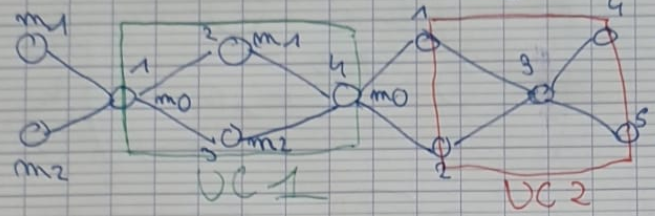
\includegraphics[scale=.5]{photo28.png}
		\end{minipage}\begin{minipage}{5cm}
			Toutes les interactions sont des raideurs linéaires 1D notées $\beta$.
		\end{minipage}\\\\
		
		$\to$\begin{minipage}[t]{17cm}
			Démontrer que les deux modélisations (ie. \Vert{UC1} et \rouge{UC2}) aboutissent à la même équation de dispersion.
		\end{minipage}
	\end{exo}
	\begin{sol}$ $\\
		\underline{Notation :} \begin{minipage}[t]{15cm}
			$\alpha_i = 2\beta-\omega^2m_i$.\\
			$u_{n,i} = U_ie^{i(kna-\omega t)}$ 
		\end{minipage}\\
		
		$F_i = \beta\left(U_{n-1}+U_{n+1}-2U_n\right)$
		
		$(2\beta-\omega^2 m_i) U_i =  \beta\displaystyle\sum_{j\not=i} f_{i,j}(k)U_j = 0$
		
		\newpage
		
		\begin{minipage}{18.5cm}
			
			\[
			\mathbb{M}_1 =
			\begin{bNiceArray}{cc|cc}[first-row,last-col,margin]
				1 & 2 & 3 & 4 & \\
				m_0/2 & 0 & 0 & 0 & 1 \\
				0 & m_1 & 0 & 0 & 2 \\
				\hline
				0 & 0 & m_2 & 0 & 3 \\
				0 & 0 & 0 & m_0/2 & 4
			\end{bNiceArray}\hspace{1cm} \mathbb K_1 =\begin{bNiceArray}{cc:cc}[margin]
				2\beta & \beta & -\beta & 0 \\
				-\beta & 2\beta & 0 & -\beta \\
				\hdashline 
				-\beta & 0 & 2\beta & -\beta \\
				0 & -\beta & -\beta & 2\beta		
			\end{bNiceArray}
			\]
			
			\vspace{.5cm}
			
			\[
			\mathbb M_2 = \begin{bNiceMatrix}[first-row,last-col]
				1 & 2 & 3 & 4 & 5 & \\
				m_1/2 & & & \Block{3-2}<\large>{(0)} & & 1\\
				& m_1/2 & & & & 2 \\
				\Block{2-3}<\large>{(0)} 
				& & m_0 & & & 3 \\
				& & & m_1/2 & & 4 \\
				& & & & m_2/2 & 5
			\end{bNiceMatrix} \hspace{1cm} \mathbb K_2 = \begin{bNiceMatrix}[margin,last-col]
				\beta & 0 & \Block[draw=red]{2-1}{\begin{matrix}
						-\beta \\ -\beta
				\end{matrix}} & \Block{2-2}{(0)} & & 1 \\
				0 & \beta & & & & 2\\
				\Block[draw=red]{1-2}{} -\beta & -\beta & \Block[draw=red]{3-3}{} 4\beta & \Block[draw=black]{1-2}{} +\beta & -\beta & 3 \\
				\Block{2-2}{(0)} & & \Block[draw=black]{2-1}{} -\beta & -\beta & 0 & 4 \\
				& & -\beta & 0 & \beta & 5
			\end{bNiceMatrix}
			\]
			
			\vspace{.5cm}
			
			\[\begin{aligned}
				L = \begin{bmatrix}
					\beta & 0 \\
					0 & \beta
				\end{bmatrix} & \hspace{1cm} & R = \begin{bmatrix}
					-\beta & 0 \\
					0 & \beta
				\end{bmatrix} & \hspace{1cm} & Li = \begin{bmatrix}
					-\beta \\ - \beta
				\end{bmatrix} \\\\
				iL = \begin{bmatrix}
					-\beta & - \beta
				\end{bmatrix} & \hspace{1.5cm} & Di = \begin{bmatrix}
					4\beta
				\end{bmatrix} & \hspace{1.5cm} & LR = \begin{bmatrix}
					0 & 0 \\
					0 & 0
				\end{bmatrix} \\\\
				RL = \begin{bmatrix}
					0 & 0 \\
					0 & 0
				\end{bmatrix} & \hspace{1.5cm} & iR = \begin{bmatrix}
					-\beta & - \beta
				\end{bmatrix} & \hspace{1.5cm} & Ri = \begin{bmatrix}
					-\beta \\ - \beta
				\end{bmatrix} \\\\
				DR = \begin{bmatrix}
					-\beta & 0 \\ 0 & \beta
				\end{bmatrix}
			\end{aligned}\]
			
			\vspace{.5cm}
			
			$t_\lambda(M) = \begin{bmatrix}
				M_{RL}\frac1\lambda M_L+M_R+M_{LR}\lambda & M_{Ri}\frac1\lambda + M_{Li} \\
				M_{iL}+M_{iR}\lambda & M_i
			\end{bmatrix}$ et $\mathbb M = \begin{bNiceMatrix}[margin=1em]
				m_0 & & 0 & 0 \\\\
				0 & & m_1 & 0 \\
				0 & & 0 & m_2
				\CodeAfter
				\SubMatrix[{1-1}{1-1}]
				\SubMatrix[{1-3}{1-4}]
				\SubMatrix[{3-1}{4-1}]
				\SubMatrix[{3-3}{4-4}]
			\end{bNiceMatrix}$\\
			$t_\lambda(K) = \begin{bNiceMatrix}[margin=1em]
				4 & & (1+\lambda) & -1 & -1 \\\\
				\Block{2-1}{(1+\lambda)} & -1 &  &2 & 0 \\
				& -1 & & 0 & 2
				\CodeAfter
				\SubMatrix[{1-4}{1-5}]
				\SubMatrix[{3-4}{4-5}]
				\SubMatrix[{3-2}{4-2}]
			\end{bNiceMatrix}$\\
			
			L'équation de dispersion "augmenté" ($\omega(k)$) :
			
			\[
			\left(\beta \begin{bmatrix}
				4 & -(1+\lambda) & -(1+\lambda) \\
				-(1+\lambda) & 2 & 0 \\
				-(1+\lambda) & 0 & 2
			\end{bmatrix} - \omega^2 \begin{bmatrix}
				m_0 \\
				& m_1 \\
				& & m_2
			\end{bmatrix}\right)\begin{bmatrix}
				U_1 \\ U_2 \\ U_3
			\end{bmatrix} = \begin{bmatrix}
				0 \\ 0 \\ 0
			\end{bmatrix}
			\]
		\end{minipage}		
	\end{sol}
	
	
	\subsection{Dynamique des systèmes périodiques (section 3 - ...)}
	
	\begin{exo}
		\begin{minipage}[t]{15cm}
			On suppose que $\begin{cases}
				a=0\\ b=L
			\end{cases}$ et $\begin{cases}
				V_a(\omega)=0\\ V_b(\omega) = V
			\end{cases}$
		\end{minipage}\\
		Démontrer que $U(t,x) = \dfrac V{\sqrt{2\pi}}\displaystyle\int_\R \dfrac{\sin(k(\omega)x)}{\sin(k(\omega)L)} e^{i\omega t}\mathrm d\omega$
	\end{exo}	
	\begin{sol}
		$\forall \omega \begin{aligned}[t]
			\begin{cases}
				U(\omega,0) = 0 \\
				U(\omega,L) = V
			\end{cases} &\iff \begin{cases}
				A^+e^{-ik.0}+A^-e^{ik.0} = 0 \\
				A^+e^{-ikL}+A^-e^{ikL} = V
			\end{cases}\\
			&\iff \begin{bmatrix}
				1 & 1\\
				e^{-ikL} & e^{ikL}
			\end{bmatrix}\begin{bmatrix}
				A^+\\ A^-
			\end{bmatrix} = \begin{bmatrix}
				0 \\ V
			\end{bmatrix}\\
			&\iff \begin{bmatrix}
				A^+ \\ A^-
			\end{bmatrix} = \dfrac V{e^{ikL}-e^{-ikL}}\begin{bmatrix}
				-1 \\ 1
			\end{bmatrix}
		\end{aligned}$\\
		
		$U(\omega,x) = \dfrac{-Ve^{ikx}}{e^{ikL}-e^{-ikL}} + \dfrac{Ve^{ikx}}{e^{ikL}-e^{-ikL}} = \dfrac{\sin(kx)}{\sin(kL)}V$\\
		Or $U(t,x) = \dfrac1{\sqrt{2\pi}}\displaystyle\int_{-\infty}^{+\infty} U(\omega,x) e^{i\omega t}\mathrm d\omega = \dfrac V{\sqrt{2\pi}}\displaystyle\int_\R \dfrac{\sin(kx)}{\sin(kL)}\mathrm d\omega$
	\end{sol}
	
	\begin{exo}[applicatif] 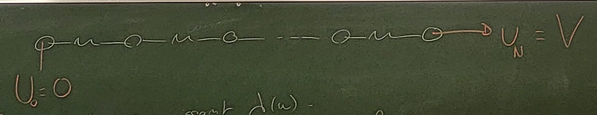
\includegraphics[scale=.5]{photo31.png}\\
		\begin{enumerate}[label=$\cdot$]
			\item Pour tout $\omega$, calculer $U_n(\omega)$, connaissant $\lambda(\omega)$.
			\item Comparer la solution à la solution similaire pour la corde finie.
		\end{enumerate}
	\end{exo}
	\begin{sol}
		\underline{Rappel :} dans un système à 1 degré de liberté et une onde, la décomposition en ondes (de Bloch) s'écrit : $\forall n\in \N$, $u_n = \lambda^n A^+ + \lambda^{N-n}A^-$.\\
		
		$\begin{aligned}
			\begin{cases}
				U_0 = 0 \\
				U_N = V
			\end{cases} \iff \begin{cases}
				\lambda^0 A^+ + \lambda^N A^- = 0\\
				\lambda^N A^+ + \lambda^0 A^- = V
			\end{cases} &\iff \begin{cases}
				A^+ = -\lambda^N A^-\\
				-\lambda^NA^- + A^- = V
			\end{cases}\\
			& \iff \begin{cases}
				A^+ = -\lambda^N \dfrac V{-\lambda^N+1}\\
				A^- = \dfrac V{-\lambda^N+1}
			\end{cases}
		\end{aligned}$\\
		
		Ainsi $\begin{bmatrix}
			1 & \lambda^N \\
			\lambda^N & 1
		\end{bmatrix}\begin{bmatrix}
			A^+ \\ A^-
		\end{bmatrix} = \begin{bmatrix}
			0 \\ V
		\end{bmatrix}$\\
		
		$\implies\begin{bmatrix}
			A^+ \\ A^-
		\end{bmatrix} = \dfrac1{1-\lambda^{2N}}\begin{bmatrix}
			1 & - \lambda^N \\
			-\lambda^N & 1
		\end{bmatrix}\begin{bmatrix}
			0 \\ V
		\end{bmatrix}$\\
		
		Donc $\begin{bmatrix}
			A^+ \\ A^-
		\end{bmatrix} = \dfrac V{1-\lambda^{2N}}\begin{bmatrix}
			-\lambda^N \\ 1
		\end{bmatrix}$\\
		On retrouve les déplacements $\begin{aligned}[t]
			U_n & = \lambda^n \dfrac{-\lambda^N}{1-\lambda^{2N}}V + \lambda^{N-n}\dfrac1{1-\lambda^{2N}}V \\
			& = \dfrac{\lambda^{N-n} - \lambda^{N+1}}{\lambda^N(\lambda^{-N}-\lambda^N)}V \\
			&= \dfrac{\lambda^{-n}-\lambda^n}{\lambda^{-N}-\lambda^N}V
		\end{aligned}$\\
		\begin{minipage}[t]{15cm}
			Or $\begin{cases}
				\lambda = e^{-ika} \\
				L = Na
			\end{cases}$, donc $U_n = \dfrac{\sin(kL\frac nN)}{\sin(kL)}V$ 
			, où $k(\omega)=\frac i\alpha\ln\left(1-\frac{2\omega^2}{\omega_0} - \frac{2\omega}{\omega_0}\sqrt{\frac{\omega^2}{\omega_0^2}-1}\right)$\\
			
			Pour la corde (uniforme) de longueur $L$, nous avions : $U(x) = \dfrac{\sin(kx)}{\sin(kL)} V$
		\end{minipage}	
	\end{sol}
	
	\begin{exo}
		\begin{minipage}[t]{14cm}
			Écrire les systèmes analogues pour les conditions aux limites de type $(U_0-F_N)$ et $(F_0-U_N)$
		\end{minipage}
		
		\begin{minipage}[t]{18cm}
			Puis appliquer au système suivant : \hspace{.5cm} 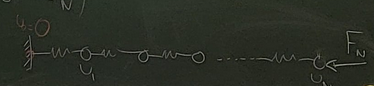
\includegraphics[scale=.5]{photo35.png}
		\end{minipage}
	\end{exo}
	\begin{sol}$ $\\
		\begin{minipage}[t]{18cm}
			La décomposition en ondes de Bloch s'écrit : $\forall n \in [\![0,N]\!], u_n = \underline{\underline{\Phi}}^+\underline{\underline{\Lambda}}^N \underline{a}^+ + \underline{\underline{\Phi}}^-\underline{\underline{\Lambda}}^{N-1}\underline{a}^-$\\
			Le système global s'écrit en fonction de la matrice dynamique $\mathbb D = \mathbb K - \omega^2 \mathbb M = \begin{bmatrix}
				D_{L} & D_{LR} \\
				D_{RL} & D_L
			\end{bmatrix}$\\
			\begin{minipage}{13cm}
				$\begin{bmatrix}
					D_L && D_{LR} \\
					D_{RL} && D_R+D_L & \ddots \\
					&\ddots  && \ddots & \ddots \\
					&& \ddots && \ddots & \ddots\\
					&&& D_{RL}  & D_L+D_R && D_{LR} \\
					&&&		 & D_R		&& D_R
				\end{bmatrix}\begin{bmatrix}
					\rouge{u_0} \\
					\bleu{u_1} \\
					\vdots\\
					\vdots\\
					\bleu{u_{N-1}} \\
					\bleu{u_N}
				\end{bmatrix} = \begin{bmatrix}
					\bleu{f_0}\\
					\vdots\\
					\vdots\\
					\vdots\\
					\vdots\\
					\rouge{F_N}
				\end{bmatrix}$
			\end{minipage} \begin{minipage}{2cm}
				\bleu{inconnu}\\
				\rouge{connu}
			\end{minipage}\\
			Les conditions aux limites sont : $\begin{cases}
				u_0 = U_0 & \text{à gauche }\\
				D_{RL}u_{N-1}+D_Ru_N = F_N & \text{à droite}
			\end{cases}$\\
			$\begin{cases}
				\Phi^+ a^+ + \Phi^-\Lambda^Na^- = U_0\\
				(D_{RL}\Phi^+\Lambda^{N-1}+D_R\Phi^+\Lambda^N)a^+ + (D_{RL}\Phi^-\Lambda+D_R\Phi^-)a^- = F_N
			\end{cases}$
		\end{minipage}
		
		\begin{minipage}{18cm}
			ce qui donne le système : $\begin{bmatrix}
				\Phi^+ & \Phi^-\Lambda^N \\
				D_{RL}\Phi^+\Lambda^{N-1}+D_R\Phi^+\Lambda^N & D_{RL}\Phi^-\Lambda+D_R\Phi^-
			\end{bmatrix}\begin{bmatrix}
				a^+ \\ a^-
			\end{bmatrix} = \begin{bmatrix}
				U_0\\ F_N
			\end{bmatrix}$\\
			Appliquons à la chaîne mono finie en condition U-F :\\
			$\begin{cases}
				\Phi^+ = \Phi^- = 1 \\
				\Lambda = \lambda
			\end{cases}$, \begin{minipage}[t]{15cm}
				cellule : 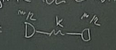
\includegraphics[scale=.5]{photo36.png}\\
				$\mathbb D = \mathbb K - \omega^2 \mathbb M = \begin{bmatrix}
					k & -k \\
					-k & k
				\end{bmatrix} - \omega^2\begin{bmatrix}
					m/2 & 0 \\
					0 & m/2
				\end{bmatrix} = \begin{bmatrix}
					k-\omega^2 m/2 & -k \\
					-k & k-\omega^2m/2
				\end{bmatrix}$
			\end{minipage}\\
			
			Le système devient : $\begin{bmatrix}
				1 & \lambda^N \\
				-k\lambda^{N-1}+(k-\omega^2m/2)\lambda^N & -k\lambda+(k-\omega^2m/2)
			\end{bmatrix}\begin{bmatrix}
				a^+ \\ a^-
			\end{bmatrix} = \begin{bmatrix}
				0 \\ F_N
			\end{bmatrix}$ car $U_0 = 0$\\
			
			$\begin{aligned}
				(L1) & a^+ + \lambda^Na^- = 0 \implies a^- = -\lambda^N a^+ \\
				(L2) & \left[\lambda^{N-1}(\lambda k - \omega^2m/2 \lambda - k) - \lambda^{-N}(k-\omega^2m/2-\lambda k)\right]a^+ = F_N
			\end{aligned}$\\
			
			$\left(\lambda^N k - \lambda^N\omega^2m/2 - \lambda^{N-1}k-\lambda^{-N}k + \lambda^{-N}\omega^2m/2+\lambda^{-N+1}k\right) = F_N$\\
			$\left[\underbrace{\lambda^N\left(k-\omega^2m/2 - \frac k\lambda\right) - \lambda^{-N}\left(k-\omega^2m/2-k\lambda\right)}_{\alpha}\right]a^+ = F_N$\\
			Donc $\begin{cases}
				a^+ = \alpha^{-1}F_N \\
				\alpha^- = -\lambda^{-N}\alpha^-F_N
			\end{cases}$\\
			Donc la solution est : $\forall n, \begin{aligned}
				u_n &= \left(\lambda^n - \lambda^{N-n}\lambda^N\right)\alpha^{-1}F_N\\
				&=\left(\lambda^n-\lambda^{-n}\right)\alpha^{-1}F_N
			\end{aligned}$
		\end{minipage}
	\end{sol}
	
	\begin{exo}
		$ $	\\
			\begin{minipage}[t]{18cm}Assemblage de système matriciels :\\
			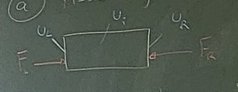
\includegraphics[scale=.5]{photo37.png}\\
			On décompose ce système en 3 domaines (ou 3 groupes de DDL après discrétisation éléments finis)\\
			L'équilibre dynamique de cet élément s'écrit : $\mathbb D\begin{bmatrix}
				u_L \\ u_i \\ u_R
			\end{bmatrix} = \begin{bmatrix}
			F_L\\ 0 \\ F_R
			\end{bmatrix}$\\
			Écrire l'assemblage de deux cellules différentes, décrites par leur raideur dynamique,\\
			notées $\mathbb D^{(1)}$ et $\mathbb D^{(2)}$\\
			
			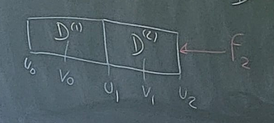
\includegraphics[scale=.5]{photo38.png}
			\end{minipage}
	\end{exo}
	\begin{sol}$ $\\
		
		 \begin{minipage}[t]{15cm}
				$\begin{bmatrix}
				D_L^{(1)} & D_{Li}^{(1)} & D_{LR}^{(1)} \\
				D_{iL}^{(1)} & D_i^{(1)} & D_{iR} \\
				D_{RL}^{(1)} & D_{Ri}^{(1)} & D_R^{(1)}+\rouge{D_L^{(2)}} & \rouge{D_{Li}^{(2)}} & \rouge{D_{LR}^{(2)}} \\
				& & \rouge{D_{iL}^{(2)}} & \rouge{D_i^{(2)}} & \rouge{D_{iR}^{(2)}} \\
				& & \rouge{D_{RL}^{(2)}} & \rouge{D_{Ri}^{(2)}} & \rouge{D_R^{(2)}}
			\end{bmatrix}\begin{bmatrix}
			U_0 \\ V_0 \\ U_1 \\ V_1\\ U_2
			\end{bmatrix} = \begin{bmatrix}
			0 \\ 0 \\ 0 \\ 0 \\ F_2
			\end{bmatrix}$
			\end{minipage}
	\end{sol}
	
	\begin{exo}$ $\\
		Guide d'ondes périodique \underline{semi-infini}\\
		\begin{minipage}{6cm}
			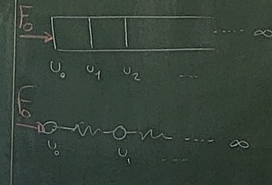
\includegraphics[scale=.5]{photo39.png}
		\end{minipage}\begin{minipage}{15cm}
			\begin{enumerate}
				\item Écrire le système global, en notant $\mathbb D = \begin{bmatrix}
					D_L & D_{LR} \\
					D_{RL} & D_R
				\end{bmatrix}$
				
				\item Décomposer en ondes et en déduire la solution $u_n$, $\forall n \in \N$
				
				\item Appliquer à une chaîne mono-atomique
			\end{enumerate}
		\end{minipage}
	\end{exo}
	\begin{sol}$ $\\
		\begin{enumerate}
			\item $\begin{bmatrix}
				D_L & D_{LR} \\
				D_{RL} && D_R + D_L && D_{LR} & \\
				&\ddots& &\ddots& &\ddots\\
				&&\ddots &&\ddots &&\ddots
			\end{bmatrix}\begin{bmatrix}
				u_0 \\ u_1 \\ u_2 \\ \vdots
			\end{bmatrix} = \begin{bmatrix}
				F_0 \\ 0 \\ 0 \\ \vdots
			\end{bmatrix}$
			
			\item $F_0 - U_n$\\
			$D_LU_0 + D_{LR} U_L = F_0$\\
			$U_0 = \Phi^+ a^+ + 0 \to$ milieu semi-uniforme\\
			$U_n = \Phi^+\Lambda a^+$\\
			$\left(\underbrace{D_L\Phi^++D_{LR}\Phi^+\Lambda}_H\right) = F_0$\\
			$a^+ = H^{-1}F_0$\\
			$U_n = \Phi^+\Lambda^n a^+ = \fbox{$\Phi^+\Lambda^n H^{-1} F_0$}$
			
			\item Appliquons avec \begin{minipage}{5cm}
				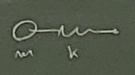
\includegraphics[scale=.5]{photo40.png}
			\end{minipage}\\
			\begin{minipage}[t]{18cm}
				$\begin{cases}
				\Phi^+ = 1 & \Lambda = \lambda\\
				\mathbb D = \begin{bmatrix}
					k-\omega^2 m & -k \\
					-k & k
				\end{bmatrix}
			\end{cases} \implies \begin{aligned}[t]
			u_n&= \Phi^+ \Lambda^n\left[D_L\Phi^+ + D_{LR}\Phi^+\Lambda\right]^{-1}\\
			&=\lambda^n\left(k-\omega^2m-k\lambda\right)^{-1}F_0
			\end{aligned}$
			\end{minipage}\\
			Donc $\forall n, \fbox{$u_n = \dfrac{\lambda^n F_0}{k-\omega^2m-k\lambda}$}$
		\end{enumerate}
		
		\vspace{-.5cm}
		
	\end{sol}
	
\end{document}